



%----------------------------------------------------------------------------------------

\newpage

% Section : Reproducibility


\section{Reproducibility}{Reproductibilité et ouverture}

\label{sec:reproducibility}


%----------------------------------------------------------------------------------------



\bpar{
The strength of science comes from the cumulative and collective nature of research, as progresses are made as Newton said ``standing on the shoulder of giants'', meaning that the scientific enterprise at a given time relies on all the work done before and that advances would not be possible without constructing on it. It includes development of new theories, but also extension, testing or falsifiability of previous ones.
}{
La production de connaissance scientifique trouve ses fondements dans la nature cumulative et collective de la recherche, puisque les progrès sont faits lorsque, comme \noun{Newton} l'a bien dit, on ``se tient sur les épaules de géants'', au sens que l'entreprise scientifique à un temps donné repose sur l'ensemble du travail précédent et qu'aucune avancée ne serait possible sans construire dessus. Cela inclut le développement de nouvelles théories, mais aussi l'extension, le test et la falsification de précédentes : l'avancée dans la construction de la tour signifie aussi la déconstruction de certaines briques obsolètes. Cet aspect de validation par les pairs et de remise en question constante est aussi ce qui légitime la science pour une connaissance plus robuste et un progrès sociétal basés sur une connaissance d'un univers objectif, par rapport aux systèmes dogmatiques qu'ils soient politiques ou religieux~\cite{bais2010praise}. % note : pourrait introduire Monod ethique de la connaissance, pas le point.
}



\bpar{
The effective practice of reproducibility seems to be increasing~\cite{stodden2010scientific} and technical means to achieve it are always more developed (as e.g. ways to make data openly available, or to be transparent on the research process such as \texttt{git}~\cite{ram2013git}, or to integrate document creation and data analysis such as \texttt{knitr}~\cite{xie2013knitr}), at least in the field of modeling and simulation. However, the devil is indeed in the details and obstacles judged at first sight as minor become rapidly a burden for reproducing and using results obtained in some previous researches. We describe two cases studies where models of simulation are apparently highly reproducible but unveil as puzzles on which research-time balance is significantly under zero, in the sense that trying to exploit their results may cost more time than developing from scratch similar models.
}{
La reproductibilité semble être de plus en plus pratiquée de manière effective~\cite{stodden2010scientific} et les moyens techniques pour l'achever sont toujours plus développés (comme par exemple les outils pour déposer les données ouvertes, ou pour être transparent dans le processus de recherche comme \texttt{git}~\cite{ram2013git}, ou pour intégrer la création de document et l'analyse de données comme  \texttt{knitr}~\cite{xie2013knitr}), au moins dans le champ de la modélisation et de la simulation. Cependant le diable est bien dans les détails et des obstacles jugés dans un premier temps comme mineurs peuvent rapidement devenir un fardeau pour reproduire et utiliser des résultats obtenus dans des recherches précédentes. Nous décrivons deux études de cas où les modèles de simulation sont en apparence hautement reproductibles mais se révèlent vite des puzzles pour lesquels l'équilibre de temps de recherche passe rapidement sous zéro, au sens où essayer d'exploiter leur résultats coûtera plus en temps que de développer entièrement des modèles similaires.
}




%%%%%%%%%%%%%%%%%%%%%%%%%%%%%%%%%%
\subsection{Explicitation, documentation and implementation of models}{Explicitation, documentation et implémentation des modèles}




%%%%%%%%%%%%%%%%%%%%%%%%%%%%%%%%%%
\subsubsection{On the Need to Explicit the Model}{Sur le Besoin d'expliciter le modèle}


\bpar{
A current myth (to which we ourselves struggle to escape indeed) is that providing entire source code and data will be a sufficient condition for reproducibility. It will work if the objective is to produce exactly same plots or statistical analysis, assuming that code provided is the one which was indeed used to produce the given results. It is however not the nature of reproducibility. First, results must be as much implementation-independent as possible for clear robustness purposes. Then, in relation with the precedent point, one of the purposes of reproducibility is the reuse of methods or results as basis or modules for further research (what includes implementation in another language or adaptation of the method), in the sense that reproducibility is not replicability as it must be adaptable~\cite{drummond2009replicability}.
}{
Un mythe à la vie dure (auquel nous essayons en fait nous-même d'échapper) est que fournir le code source complet et les données seront une condition suffisante pour la reproductibilité, puisque la reproductibilité computationnelle complète implique un environnement similaire ce qui devient vite ardu à produire comme le montrent \cite{2016arXiv160806897H}. Pour résoudre ce problème, \cite{10.1371/journal.pone.0152686} propose l'utilisation de conteneurs Dockers qui permet de reproduire même le comportement de logiciels avec interface graphique indépendamment de l'environnement. C'est d'ailleurs l'une des direction courantes de développement d'OpenMole, pour simplifier le packaging des bibliothèques et des modèles en binaire (voir l'entretien avec \noun{R. Reuillon}). Dans tous les cas, la reproductibilité a des dimensions supplémentaires, il ne s'agit pas de l'objectif unique qui serait de produire exactement les mêmes graphes et analyses statistiques, en supposant que le code fournit est celui qui a été effectivement utilisé pour produire les résultats donnés. Tout d'abord, ceux-ci doivent être autant que possible indépendants de l'implémentation~\cite{crick2017reproducibility} (c'est à dire du langage, des bibliothèques, des choix de structures de données et de type de programmation) pour des motifs clairs de robustesse. Ensuite, en relation avec le point précédent, un des buts de la reproductibilité est la réutilisation des méthodes ou résultats comme base ou modules pour une recherche future (ce qui comprend une implémentation dans un autre langage ou une adaptation de la méthode), au sens que la reproductibilité n'est pas la possibilité stricte de répliquer car elle doit être adaptable~\cite{drummond2009replicability}.
}

% note : \cite{crick2017reproducibility} recommandations plus larges


\bpar{
Our first case study fits exactly that scheme, as it was undoubtedly aimed to be shared with and used by the community since it is a model of simulation provided with the Agent-Based simulation platform NetLogo~\cite{wilensky1999netlogo}. The model is also available online~\cite{de2007netlogo} and is presented as a tool to simulate socio-economic dynamics of low-income residents in a city based on a synthetic urban environment, generated to be close in stylized facts from the real town of Tijuana, Mexico. Beside providing the source code, the model appears to be poorly documented in the literature or in comments and description of the implementation. Comments made thereafter are based on the study of the urban morphogenesis part of the model (setup for the ``residential dynamics'' component) as it is our global context of study%~\cite{raimbault2014vers} % not really citable ?
. In the frame of that study, source code was modified and commented, which last version is available on the repository of the project\footnote{at \texttt{https://github.com/JusteRaimbault/CityNetwork/tree/master/Models/Reproduction/UrbanSuite}}.
}{
Notre premier cas d'étude suit exactement ce schéma, puisqu'il a sans aucun doute été conçu pour être partagé avec la communauté et utilisé, s'agissant d'un modèle de simulation fournit avec la plateforme de modélisation agent NetLogo~\cite{wilensky1999netlogo}. Le modèle est également disponible en ligne~\cite{de2007netlogo} et est présenté comme un outil pour simuler les dynamiques socio-économiques des résidents à bas revenus d'une ville au sein d'un environnement urbain synthétique, généré pour ressembler en terme de faits stylisés à la ville réelle de Tijuana au Mexique. Globalement, le modèle fonctionne de la façon suivante : (i) à partir de centres urbains, une distribution d'usage du sol est générée par modélisation procédurale similaire à \cite{lechner2006procedural}, c'est à dire des routes sont générées de proche en proche selon des règles géométriques et de hiérarchie locales, et un usage du sol ainsi qu'une valeur est attribué en fonction des caractéristique de la cellule (distance au centre, à la route) ; (ii) dans cet environnement urbain sont simulées des dynamiques résidentielles de migrants, qui cherchent à optimiser une fonction d'utilité dépendant du coût de la vie et de la configuration des autres migrants. À part fournir le code source, le modèle n'est que peu documenté dans la littérature ou dans les commentaires et la description de l'implémentation. Les commentaires qui suivent sont basés sur l'étude de la partie du modèle simulant la morphogenèse urbaine (initialisation pour la composante ``dynamiques résidentielles'') comme il s'agit de notre contexte global d'étude. Dans le cadre de cette étude, le code source a été modifié et commenté, dont la dernière version est disponible sur le dépôt du projet\footnote{À \url{https://github.com/JusteRaimbault/CityNetwork/tree/master/Models/Reproduction/UrbanSuite}.}.
}



\paragraph{Rigorous Formalization}{Formalisation rigoureuse}


\bpar{
An obvious part of model construction is its rigorous formalization in a formal framework distinct from source code. There is of course no universal language to formulate it~\cite{banos2013pour}, and many possibilities are offered by various fields (e.g. UML, DEVS, pure mathematical formulation). No paper nor documentation is provided with the model, apart from the embedded NetLogo documentation, that only thematically describes in natural language the ideas behind each step without developing more and provides information about role of different elements of the interface.
}{
Une partie évidente de la construction d'un modèle est sa formalisation rigoureuse dans un cadre formel distinct du code source. Il n'y a bien sûr aucun langage universel pour le formuler~\cite{banos2013pour}, et de nombreuses possibilités sont offertes par de nombreux champs (e.g. UML, DEVS, formulation mathématique pure), mais l'étape de formalisation précise, qui suit généralement une description plus intuitive donnant les idées et processus dominants, ne peut pas être sautée. On pourrait se dire que le code source y est équivalent, mais ce n'est pas exactement vrai car on pourrait alors ne plus distinguer certains choix d'implémentation de la structure du modèle. Aucun article ni documentation n'accompagne le modèle ici, au delà de la documentation embarquée NetLogo, qui ne décrit que de manière thématique en langage naturel les idées derrière chaque étape sans plus développer et fournit de l'information sur le rôle des différents éléments de l'interface. Comme ces éléments manquent ici, le modèle n'est guère utilisable tel quel. On pourrait nous objecter ici que la partie que nous étudions est une procédure d'initialisation et non le coeur du modèle : nous maintenons que l'ensemble des procédures doit être également documenté et implémenté avec un soin équivalent, ou pointer vers une référence extérieure dans le cas d'utilisation d'un modèle tiers, comme nous le faisons d'ailleurs pour le couplage effectué en~\ref{sec:computation}.
}



\bpar{
This formulation is a key for it to be understood, reproduced and adapted; but it also avoids implementation biases such as
\begin{itemize}
\item Architecturally dangerous elements: in the model, world context is a torus and agents may ``jump'' in the euclidian representation, what is not acceptable for a 2D projection of real world. To avoid that, many tricky tests and functions were used, including unadvised practices (e.g. dead of agents based on position to avoid them jumping).
\item Lack of internal consistence: the example of the patch variable \texttt{land-value} used to represent different geographical quantities at different steps of the model (morphogenesis and residential dynamics), what becomes an internal inconsistence when both steps are coupled when option \texttt{city-growth?} is activated.
\item Coding errors: in an untyped language such as NetLogo, mixing types may conduct to unexpected runtime errors, what is the case of the patch variable \texttt{transport} in the model (although no error occurs in most of run configurations from the interface, what is more dangerous as the developer thinks implementation is secure). Such problems should be avoided if implementation is done from an exact formal description of the model.
\end{itemize}
}{
Une telle formulation est essentielle pour que le modèle soit compris, reproduit et adapté ; mais elle évite également des biais d'implémentation comme :
\begin{itemize}
\item Des éléments architecturaux dangereux : le contexte du monde est une sphère, ce qui n'est pas raisonnable pour ce modèle à l'échelle d'une ville, les mesures de proximité jouant un rôle important dans les processus de production de la forme urbaine. Les agents peuvent passer d'un côté du monde à l'autre dans la représentation euclidienne, ce qui n'est pas acceptable pour une projection en deux dimensions du monde réel. Pour éviter cela, de nombreux tests et fonctions subtiles sont utilisés, incluant des pratiques déconseillées (e.g. mort d'agents basée sur leur position pour les empêcher de sauter).
\item Manque de cohérence interne : par exemple la variable de cellule \texttt{land-value} (non documentée mais dont l'utilisation se reconstruit par analyse du code) utilisée pour représenter différentes quantités géographiques à différentes étapes du modèle (morphogenèse et dynamiques résidentielles), ce qui devient une incohérence interne quand les deux étapes sont couplées lorsque l'option permettant de faire croître la ville est activée.
\item Erreur de code : dans un langage non typé comme NetLogo, le mélange des types peut conduire à des erreurs inattendues à l'execution, ou même des \emph{bugs} non détectables directement et alors plus dangereux. C'est le cas de la variable de patch \texttt{transport} dans le modèle (même si aucune erreur ne survient dans la majorité des configurations depuis l'interface, ce qui est plus dangereux comme le développeur pense que l'implémentation est sûre). De tels problèmes devraient être évités si l'implémentation est faite à partir d'une description exacte du modèle.
\end{itemize}
}



\paragraph{Transparent Implementation}{Implémentation transparente}


\bpar{
A totally transparent implementation is expected, including ergonomics in architecture and coding, but \ldots
}{
Une implémentation totalement transparente doit être attendue, incluant une certaine ergonomie dans l'architecture et le code, mais aussi dans l'interface et la description du comportement attendu du modèle.
}

\paragraph{Expected Model Behavior}{Comportement attendu du modèle}


\bpar{
Whatever the definition, a model can not be reduced to its formulation and/or implementation, as expected model behavior or model usage can be viewed as being part of the model itself. In the frame of \noun{Giere}'s perspectivism~\cite{giere2010scientific}, the definition of model includes the purpose of use but also the agent who aims to use it. Therefore a minimal explication of model behavior and exploration of parameter roles is highly advised to decrease chances of misuses or misinterpretations of it. It includes simple runtime charts that are immediate on the NetLogo platform, but also indicators computations to evaluate outputs of the model. It can also be improved visualizations during runtime and model exploration, such as showed in Fig.~\ref{fig:example_tij_viz}.
}{
Quelle que soit la définition, un modèle ne peut pas être réduit à sa formulation et/ou implémentation, comme le comportement attendu ou l'utilisation du modèle peuvent être vu comme des parties du modèle lui-même. Dans le cadre du perspectivisme de \noun{Giere}~\cite{giere2010scientific}, la définition du modèle inclut le motif de l'utilisation mais aussi l'agent qui vise à l'utiliser. Pour cela une explication minimale du comportement du modèle et une exploration du rôle des paramètres sont fortement recommandés pour diminuer les chances de mauvais usage ou mauvaises interprétations de celui-ci. Cela inclut des graphes simples obtenus immédiatement à l'exécution sur la plateforme NetLogo, mais aussi un calcul d'indicateurs pour évaluer les sorties du modèle. Il peut aussi s'agir de visualisations améliorées pendant l'execution et l'exploration du modèle, comme le montre la figure~\ref{fig:reproducibility:tijuana}.
}


%%%%%%%%%%%%%%%%%%%%%
\begin{figure}
%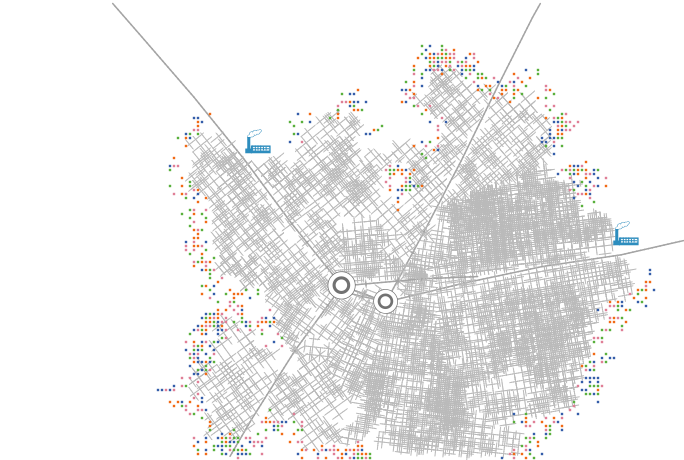
\includegraphics[width=0.3\linewidth]{Figures/Reproducibility/stdView}
%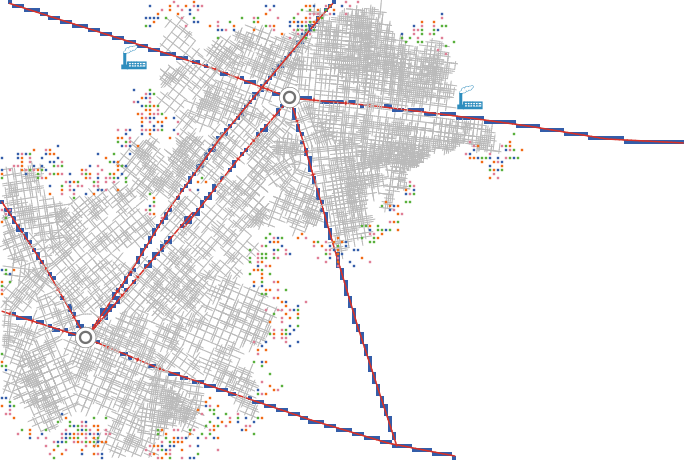
\includegraphics[width=0.3\linewidth]{Figures/Reproducibility/ViewRoads}
%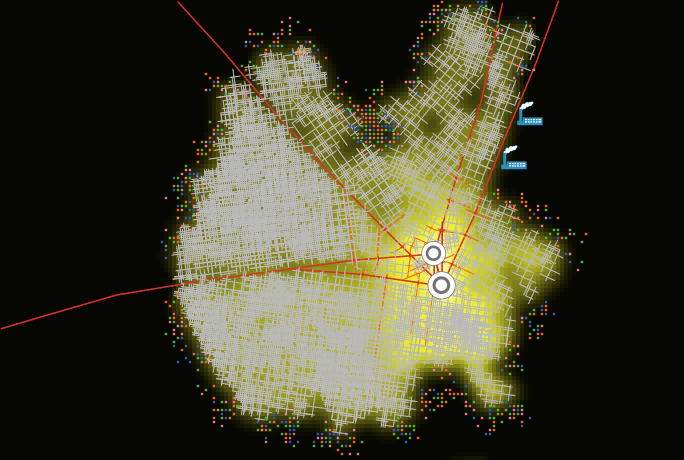
\includegraphics[width=0.3\linewidth]{Figures/Reproducibility/landValues_cityFinished}
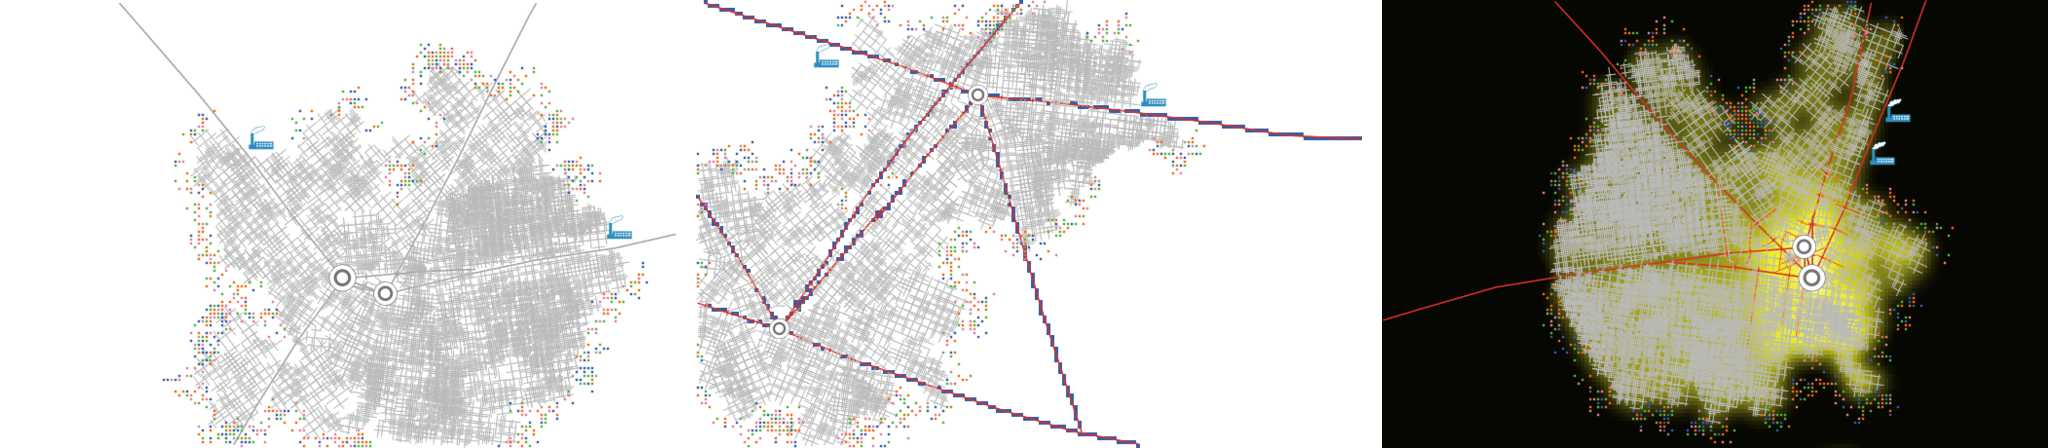
\includegraphics[width=\linewidth]{Figures/Final/3-1-3-fig-reproducibility-tijuana.jpg}
\caption[Reproducibility and visualization][Reproductibilité et visualisation]{Example of simple improvement in visualization that can help understanding mechanisms implied in the model. \textit{Left: } Example of original output ; \textit{Middle: } Visualization of main roads (in red) and underlying patches attribution, suggesting possible implementation bias in the use of discretized trace of roads to track their positions ; \textit{Right: }Visualization of land values using a more readable color gradient. This step confirms the hypothesis, through the form of value distribution, that the morphogenesis step is an unnecessary detour to generate a random field for which simple diffusion method should provide similar results, as detailed in the paragraph on implementation.\label{fig:reproducibility:tijuana}}{\textbf{Exemple d'amélioration simple dans la visualisation qui peut aider à appréhender les mécanismes impliqués par le modèle.} (Gauche) Exemple de sortie originale ; (Centre) Visualisation des routes principales (en rouge) et de l'attribution des patches sous-jacente, qui suggère de possibles biais d'implémentation dans l'utilisation de la trace discrete des routes pour garder trace de leur position ; (Droite) Visualisation des valeurs foncières en utilisant un gradient de couleur plus lisible. Cette étape confirme l'hypothèse, par la forme de la distribution des valeurs, que l'étape de morphogenèse est un détour non-nécessaire pour générer un champ aléatoire pour lequel des simples mécanismes de diffusion devrait fournir des résultats similaires, comme détaillé dans le paragraphe sur l'implémentation. Initialement, l'interface du modèle ne permet pas ces options de visualisation, ces à dire se limite à la première image. On ne peut se rendre compte des processus en jeu pour la morphogenèse, liés aux patches de route et au valeurs foncières se diffusant.\label{fig:reproducibility:tijuana}}
\end{figure}
%%%%%%%%%%%%%%%%%%%%%



%%%%%%%%%%%%%%%%%%%%%
\subsubsection{On the Need of Exactitude in Model Implementation}{Sur le besoin d'exactitude dans l'implémentation du modèle}


\bpar{
Possible divergences between model description in a paper and the effectively implemented processes may have grave consequences on the final reproducibility. The road network growth model given in~\cite{barthelemy2008modeling} is one example of such a discrepancy. A strict implementation of model mechanisms provide slightly different results than the one presented in the paper, and as source code is not provided we need to test different hypotheses on possible mechanisms added by the programmer (that seems to be a connexion rule to intersections under a certain distance threshold). Lessons that could be possibly drawn from this examples are 
\begin{itemize}
\item the necessity of providing source code
\item the necessity of providing architecture description along with code (if model description is in a langage too far from architectural specifications) in order to identify possible implementation biaises
\item the necessity of performing and detailing explicitly model explorations, that would in that case have helped to identify the implementation bias.
\end{itemize}
}{
Des divergences potentielles entre la description du modèle dans un article et les processus effectivement implémentés peut avoir des conséquences graves sur la reproductibilité finale. Le modèle de croissance du réseau routier donné dans~\cite{barthelemy2008modeling} est un exemple d'un tel décalage. Une implémentation stricte des mécanismes du modèle\footnote{Notre implémentation en NetLogo est disponible à \url{https://github.com/JusteRaimbault/CityNetwork/tree/master/Models/Reproduction/NWGrowth/LocalDistanceMin}.} produit des résultats légèrement différents de ceux présentés dans l'article, et comme le code source n'est pas fourni nous devrions tester différentes hypothèses sur des mécanismes possibles ajoutés par le programmeur (qui semble être une règle de connexion aux intersections sous un certain seuil de distance). Des leçons qui peuvent éventuellement être tirées de cet exemple, qui rejoignent partiellement mais complètent celle tirées dans l'étude de cas précédente, sont :
\begin{itemize}
\item la nécessité de fournir le code source ;
\item la nécessité de fournir une description de l'architecture en même temps que le code (si la description du modèle est faite dans un langage trop loin de spécification architecturales) afin d'identifier des biais possibles d'implémentation ;
\item la nécessité de procéder à des explorations explicites du modèle et de les détailler, ce qui dans ce cas aurait permis d'identifier de possibles biais d'implémentation.
\end{itemize}
}



\bpar{
Making the last point mandatory may ensure a limited risk of scientific falsification as it is generally more complicated to fake false exploration results than to effectively explore the model. One could imagine an experiment to test the general behavior of a subset of the scientific community regarding reproducibility, that would consist in the writing of a false modeling paper in the spirit of~\cite{zilsel2015canular}, in which opposite results to the effective results of a given model are provided, without providing model implementation. A first bunch of test would be to test the acceptance of a clearly non-reproducible paper in diverse journals, possibly with a control on textual elements (using or not ``buzz-words'' associated to the journal, etc.). Depending on results, a second experiment may be tested with providing open source code for model implementation but still with false results, to verify if reviewers effectively try to reproduce results when they ask for the code (in reasonable computational power limits of course, HPC being not currently broadly available in Humanities).
}{
Rendre le dernier point obligatoire pourrait assurer un risque limité de falsification puisqu'il est généralement plus compliqué de falsifier des résultats d'exploration plutôt que d'explorer effectivement le modèle. On pourrait imaginer une expérience pour tester le comportement général d'un sous-ensemble de la communauté scientifique au regard de la reproductibilité, qui consisterait en l'écriture d'un faux article de modélisation dans l'esprit de \cite{zilsel2015canular}, dans lesquels des résultats opposés aux résultats effectifs d'un modèle donné seraient fournis, sans fournir l'implémentation du modèle. Un premier test serait de tester l'acceptation d'un article clairement non reproductible dans divers journaux, si possible avec un contrôle sur les éléments textuels (par exemple en utilisant ou non des ``buzz-words'' chers au journal). Selon les résultats, une expérience plus poussée serait de fournir l'implémentation open source mais toujours avec des résultats modifiés plus ou moins fortement, afin de tester si les reviewers essayent effectivement de reproduire les résultats quand ils demandent le code (dans des capacités de calcul limitées bien sûr, le calcul intensif n'étant pas encore largement disponibles en sciences sociales). Notre intuition est que les résultats obtenus seraient fortement négatifs, vu les difficultés rencontrées par une exigence de discipline de reproduction indépendante lors de nombreuses relectures, même pour des revues faisant de la reproductibilité une condition \emph{sine qua non} de la publication, les auteurs trouvant des astuces pour se dérober aux contraintes (postuler que des données de simulation ne sont pas des données, ne fournir qu'une version agrégée inutile du jeu de données utilisées, etc. ; nous reviendrons sur le rôle des données plus loin).
}






%%%%%%%%%%%%%%%%%%%%%
\subsubsection{Interactive Exploration and Production of Results}{Exploration interactive et production des résultats}

L'usage d'applications interactives pour la fouille de données a des avantages non discutables, tel qu'une familiarisation avec la structure des données par une vue d'ensemble qui serait beaucoup plus laborieuse voire impossible autrement. C'est la même idée sous-jacente qui justifie l'interactivité pour l'exploration préliminaire des modèles multi-agents intégrée à des plateformes comme Netlogo~\cite{wilensky1999netlogo} ou Gamma~\cite{drogoul2013gama}. Un objectif similaire est implicite dans~\cite{rey2015plateforme}, c'est à dire une intégration complète de l'exploration fine des modèles et de la production des graphes de sortie ainsi que leur exploration interactive. Comme le rappelle \noun{Romain Reuillon} (Entretien du 11/04/2017, voir \ref{app:sec:interviews}), la plateforme OpenMole qui devait accueillir cette couche supplémentaire était à ses débuts à l'époque et ne l'est toujours pas aujourd'hui, puisque l'état de l'art de telles pratiques est en pleine construction et bouleversements réguliers~\cite{holzinger2014knowledge}.


Des difficultés au regard de la reproductibilité, qui nous concernent particulièrement ici, sont récurrentes et loin d'être résolues. En effet, il faut bien situer la position de ces outils et méthodes comme une aide cognitive préliminaire\footnote{Que nous ne jugeons pas superficielle puisque nous les mobilisons au moins deux fois par la suite, voir ci-dessous ainsi que \ref{sec:energyprice}.}, mais peu souvent comme permettant la production de résultats finaux : lorsque les paramètres ou dimensions se multiplient, l'export d'un graphe est bien souvent déconnecté de l'information complète ayant conduit à sa production. De la même manière, l'utilisation de notebooks intégrés tel Jupyter, permettant d'intégrer analyses et rédaction du compte-rendu, peut devenir dangereux car on peut justement revenir sur un script, tester différentes valeurs d'un paramètre, et perdre les valeurs qui avaient produit un graphe donné. L'utilisation de versioning peut être une solution partielle mais souvent lourde.


Dans l'idéal, tout logiciel interactif permettant l'export de résultats devrait en même temps exporter un script ou une description exacte et utilisable permettant d'arriver exactement à ce point à partir des données brutes. La plupart des applications d'exploration interactives de données spatio-temporelles sont à ce regard relativement immatures scientifiquement, car même dans le cas où elles sont totalement honnêtes et transparentes sur les analyses présentées à l'utilisateur, ce qui n'est malheureusement pas la règle, les tâtonnements d'exploration progressive ne sont pas reproductibles et la méthode d'extraction de caractéristiques est ainsi relativement aléatoire. En poussant le raisonnement, leur utilisation révélerait plutôt l'aveu d'une faiblesse d'un manque de méthodes systématiques accompagnant la découverte de motifs dans des données spatio-temporelles complexes de manière efficace.

Par un plaidoyer visionnaire, \noun{Banos} avait déjà mis en garde contre ``les dangers de la jungle'' des données dans~\cite{banos2001propos}, quand il souligne très justement que l'exploration interactive doit nécessairement se doubler d'indicateurs locaux adaptés, mais surtout d'outils d'exploration automatisés et de critère d'évaluation des choix faits et des motifs découverts par l'utilisateur. Nous revenons encore à l'idée d'une plateforme intégrée dont OpenMole pourrait être un précurseur. La combinaison des capacités cognitives humaines au traitement machine, notamment pour des problèmes de vision par ordinateur, ouvre des possibilités de découvertes inédites, encore plus via une utilisation collective comme en témoigne le Galaxy Zoo~\cite{2010AEdRv...9a0103R}\footnote{Le principe rejoint celui de \emph{citizen science}, en faisant participer des volontaires hors de la communauté scientifique à des tâches requérant cognition mais pas de connaissances scientifique : la classification d'images, dans le but d'entraîner des algorithmes supervisés, est l'exemple initial du Galaxy Zoo pour la forme des galaxies.}. Les résultats d'un crowdsourcing de la cognition humaine peuvent rivaliser avec les techniques automatiques les plus avancées comme le montre~\cite{10.1371/journal.pone.0178165} pour l'exemple de la comparaison de cartes spatiales.


Ces possibilités ne doivent cependant pas être sur-estimées ou utilisées à mauvais escient, et les questions d'intégration efficiente homme-machine sont d'ailleurs totalement ouvertes. Dans le domaine de la visualisation de l'information géographique, \cite{pfaender2009spatialisation} introduit une sémiologie spécifique visant à favoriser l'exploration de grands jeux de données hétérogènes, et l'expérimente sur une application spécifique : il s'agit d'une avancée considérable vers une plateforme intégrée et une exploration interactive saine et reproductible, les directions d'exploration répondant à des modèles basés sur les sciences cognitives. 


Enfin, le rôle de l'interactivité dans la communication et la vulgarisation scientifiques est exploré par l'Annexe~\ref{app:sec:mediationecotox}, qui suggère la mise en place de jeux, notamment un jeu informatique interactif, pour faciliter la transmission de concepts scientifiques au public. cela nous montre que le développement de ces pratiques innovantes dépasse largement le seul cadre de l'analyse de données.



\subsubsection{Application}{Mise en application}

\bpar{
Again, reproducibility and transparency is a non-negotiable feature of contemporaneous science, along with Open practices and Open Access. Too much examples (see a very recent one in experimental economics~\cite{camerer2016evaluating}) show in various disciplines the lack of reproducibility of experiments, that is a falsification of previous results or a result in itself. Falsification is a costly practice, and even if necessary~\cite{chavalarias2005nobel}, could be made more efficient through more transparency and direct reproducibility, increase therein the global workflow of science. We develop in parallel of this thesis various tools aimed to ease reproducibility, for which an overview is given in appendix~\ref{app:workflow}.
}{
Encore une fois, la reproductibilité et la transparence sont des éléments essentiels incontournables de la science contemporaine, liés aux pratiques de science ouverte et d'accès ouvert. Beaucoup d'exemples (voir un récent en économie expérimentale dans~\cite{camerer2016evaluating}) dans diverses disciplines montrent le manque de reproductibilité des résultats des expériences, alors que celle-ci doit pouvoir conduire à une falsification ou à une confirmation de ces résultats. La falsification est une pratique coûteuse car demandant un certain investissement au détriment de sa propre recherche~\cite{chavalarias2005nobel}. Elle pourrait ainsi être rendue plus efficiente grâce à une transparence augmentée. Des outils spécialement dédiés à une reproductibilité directe, souvent permise par l'ouverture, devraient accroître la performance globale de la science. Mais l'accès ouvert a des impacts bien plus larges que la science elle-même : \cite{teplitskiy2017amplifying} montrent un transfert des connaissances scientifiques accru vers la société dans le cas d'articles ouverts, notamment par des intermédiaires comme Wikipedia.
}

Le développement et la systématisation de standards et de bonnes pratiques, de manière conjointe sur les différentes problématiques évoquées, est une condition nécessaire à une rigueur scientifique qui devrait être uniforme au travers de l'ensemble des disciplines existantes. Nous construisons par exemple des outils facilitant le flot de production scientifique, ceux-ci étant détaillés en Appendice~\ref{app:workflow}. Par exemple, pour les sciences computationnelles, on a déjà évoqué les potentialités de l'utilisation de \texttt{git} qui s'étendent en fait sans contrainte de disciplines ni de types de recherche si les bonnes adaptations sont introduites. Le suivi précis de l'ensemble des étapes d'un projet, gardé en historique offrant la possibilité de revenir à n'importe laquelle à tout moment, mais aussi de travailler de façon collaborative, plus ou moins parallèlement selon les besoins en utilisant les branches, est un exemple de service fourni par cet outil. Un exemple de bonnes pratiques d'utilisation est donné par~\cite{10.1371/journal.pcbi.1004947}.


Plus généralement, les sciences computationnelles nécessitent l'adoption de certains standards et pratiques pour assurer une bonne reproductibilité, et ceux-ci restent majoritairement à développer : \cite{wilson2017good} donne des premières pistes. Concernant la qualité des données, de nombreux efforts sont faits pour introduire des cadres de standardisation des données : par exemple~\cite{10.1371/journal.pone.0178731} décrit un cadre conceptuel visant à guider la résolution de problème récurrent liés à la qualité des données de biodiversité (comme par exemple évaluer des mesures jugeant de l'usage possible d'un jeu de données pour un problème donné). De nouvelles perspectives s'ouvrent pour des futurs cadres de traitement de données intrinsèquement ouverts et reproductibles, avec le développement de nouvelles techniques comme le \emph{blockchain}\footnote{Le \emph{blockchain} consiste en la distribution d'un graphe de transactions entre utilisateurs, celles-ci étant validées (dans le cadre historique classique de type \emph{proof-of-work}) par la résolution de problèmes cryptographiques inverses par force brute, par des agents appelés mineurs, essentiels à la robustesse de l'écosystème.}, comme proposé par~\cite{2017arXiv170706552}.




%%%%%%%%%%%%%%%%%%%%%
\subsection{Open Data}{Ouverture des données}

%\subsubsection{Data}{Données}


L'accès aux données est également un point crucial pour la reproductibilité, et sans nous y attarder car cela impliquerait des développements sur la définition, la philosophie, le droit des données etc. qui sont des sujets de recherche en eux-mêmes, nous donnons des perspectives sur les opportunités offertes par une ouverture systématique des données en recherche. En géographie, les \emph{data paper} sont une pratique inexistante, et la règle est plutôt de garder la main jalousement sur un jeu produit, capitalisant sur le fait d'être le seul à y avoir accès\footnote{Il n'existe à notre connaissance pas de travail quantifiant la proportion de données ouvertes sur l'ensemble des données produites en géographie. Cela pourrait être l'objet d'un travail d'épistémologie quantitative appliquant des techniques similaires à celles développées en chapitre~\ref{ch:modelinginteractions}. La difficulté à trouver des données ouvertes, comparée à la fréquence des publications dans les domaines concernés, suggère une validité au moins qualitative de ce fait.}.

Il est évident que la qualité et quantité des connaissances produites sera nécessairement plus grande si un jeu de données est publiquement ouvert, puisqu'au moins la même chose sera obtenue, et on peut s'attendre à une prise en main par d'autres domaines, d'autres méthodes, et donc à une plus grande richesse\footnote{Il est possible d'argumenter que le système de production scientifique est complexe, et qu'une monétarisation, compétition ou privatisation accrue de la recherche peut faire partie d'un écosystème de recherche dont les sorties pourront être jugées de qualité selon les indicateurs choisis. Ces considérations sont pertinentes, mais hors de notre portée puisque relevant d'un travail en anthropologie et sociologie des sciences. Nous postulons ici ce principe, et le considérons comme une position scientifique subjective.}.

La fermeture induira plutôt des effets négatifs, comme par exemple du temps perdu à recoder un base vectorielle donnée uniquement sous forme de carte dans un article. L'argument du temps passé comme justification à la fermeture est absurde, puisqu'au contraire, en voyant les données comme une composante à part entière de la connaissance (voir le cadre de connaissances en~\ref{sec:knowledgeframework}), le temps passé doit impliquer plus de citations, donc plus d'utilisation, ce qui passe nécessairement par l'ouverture pour des données. De même, quelle logique, sinon la même absurde de propriété des connaissances, pousse les géographes à insérer un copyright sur l'ensemble de leurs cartes mais aussi leurs figures, jusqu'à un copyright pour un simple histogramme qui s'en serait bien passé si on avait pu l'interroger, honnête de simplicité ?

L'expérience d'évaluation d'articles nous induit à réellement nous inquiéter sur la valeur donnée à l'ouverture des données par les auteurs : au bout d'une dizaine d'articles, incluant des journaux affichant comme priorité et pré-requis l'ouverture totale des données et modèles, dont un seul est seulement partiellement ouvert et l'ensemble des autres implique de croire sur parole les résultats présentés (alors qu'un des but de la revue est de contourner les biais cognitifs qu'un ou des humains ont forcément par une validation croisée qui doit se faire sur les résultats bruts et non des interprétations contenant ces biais), il est difficile de croire que des mutations profondes des pratiques ne sont pas nécessaires.


Mais en suivant l'adage de Framasoft\footnote{Réseau pour la promotion du logiciel libre, \url{https://framasoft.org/}}, ``la route est longue mais la voie est libre'', les perspectives sont nombreuses pour une évolution dont la lenteur n'est pas inéluctable. Le journal Cybergéo, pionnier des pratiques d'ouverture en sciences sociales (première revue entièrement électronique, première revue à lancer une rubrique de \emph{model papers}), lance en 2017 une rubrique \emph{data papers}\footnote{Dont l'index est disponible à \url{https://cybergeo.revues.org/28545}. Le premier article est~\cite{swerts2017database}, que nous utilisons d'ailleurs en~\ref{sec:lutecia}.} visant à inciter le développement du partage de données et de l'ouverture en géographie.


Il reste des zones grises sur lesquelles il est impossible aujourd'hui d'avoir des perspectives, notamment le droit des données. Nous avons un exemple dans les analyses que nous développerons : les données bibliographiques sont obtenues au prix d'une guerre de blocage par Google et un effort technique considérable pour la gagner (voir~\ref{sec:quantepistemo} et \ref{app:sec:cybergeo}).% ; les données immobilières proviennent d'une base propriétaire achetée avec de l'argent public, et nous pouvons profiter d'un flou du contrat pour les rendre disponibles de manière agrégées avec les résultats ; les données des stations essence utilisées en~\ref{sec:energyprice} proviennent d'une source dont la légalité ne devrait pas être creusée plus, et nous ne pouvons malheureusement pas les rendre disponibles sans prendre de risques - cet aspect n'a cependant jamais fait broncher les reviewers de l'article associé qui n'ont même pas mentionné le manque d'accès aux données.


L'ouverture implique un engagement qui fait résolument partie de nos positionnements. C'est la même idée qui soutient la construction de l'application \texttt{CybergeoNetworks}\footnote{Dont la démarche et le contexte sont détaillés en Annexe~\ref{app:sec:cybergeonetworks}. Elle est disponible en ligne à \url{http://shiny.parisgeo.cnrs.fr/CybergeoNetworks}.}, qui couple les outils présentés en~\ref{sec:quantepistemo} avec d'autres approches complémentaires d'analyse de corpus, dans le but d'encourager la réflexivité scientifique, et de mettre cet outil ouvert à la disposition d'éditeurs indépendants, pour s'émanciper de la nouvelle main mise des géants de l'édition qui à la recherche d'un nouveau modèle pour sécuriser leur profits parient sur la vente de méta-contenu et de son analyse. Heureusement, la récente loi numérique en France a gagné le bras de fer contre leur revendication d'un droit exclusif sur la fouille de texte complets.



% crowdsourcing / opendata : https://sci-hub.cc/https://www.nature.com/nature/journal/vaop/ncurrent/full/nature24621.html# microbial dna base





\subsection{Illustration by an empirical study}{Illustration par une étude empirique}



Nous proposons à présent de développer un exemple concret d'étude empirique illustrant les derniers points relevés ci-dessus et nous permettant une entrée progressive dans notre problématique. Dans le cas du trafic routier en Ile-de-France, nous menons une collecte d'un jeu de données là où il n'existe pas de source ouverte. Nous mettons également en place une application permettant son exploration interactive.


Nous avons développé en~\ref{sec:networkterritories} le concept de mobilité quotidienne comme jouant un rôle clé dans les processus d'interaction entre réseaux de transport et territoires, à une échelle que nous avons désignée par microscopique. Il est de plus candidat à la mobilisation de dynamiques co-évolutives, comme le suggère l'effet des localisations sur la congestion et réciproquement.

Ici, la mobilité sera captée par le flux de trafic, et la co-évolution s'opère entre propriétés du réseau (congestion) et localisation des agents. Nous nous intéresserons plus particulièrement à l'équilibre hypothétique des flux de trafic, répondant indirectement à des problématiques que nous détaillons ci-dessous. 



\subsubsection{Context}{Contexte}


\bpar{
Traffic Modeling has been extensively studied since seminal work by~\cite{wardrop1952road} : economical and technical elements at stake justify the need for a fine understanding of mechanisms ruling traffic flows at different scales. Many approaches with different purposes coexist today, of which we can cite dynamical micro-simulation models, generally opposed to equilibrium-based techniques. Whereas the validity of micro-based models has been largely discussed and their application often questioned, the literature is relatively poor on empirical studies assessing the stationary equilibrium assumption in the Static User Equilibrium (SUE) framework. Various more realistic developments have been documented in the literature, such as Dynamic Stochastic User Equilibrium (DSUE) (see e.g. a description by~\cite{han2003dynamic}). An intermediate between static and stochastic frameworks is the Restricted Stochastic User Equilibrium, for which route choice sets are constrained to be realistic (\cite{rasmussen2015stochastic}). Extensions that incorporate user behavior with choice models have more recently been proposed, such as~\cite{zhang2013dynamic} taking into account both the influence of road pricing and congestion on user choice with a Probit model. Relaxations of other restricting assumptions such as pure user utility maximization have been also introduced, such as the Boundedly Rational User Equilibrium described by~\cite{mahmassani1987boundedly}. In this framework, user have a range of satisfying utilities and equilibrium is achieved when all users are satisfied. It produces more complex features such as the existence of multiple equilibria, and allows to account for specific stylized facts such as irreversible network change as developed by~\cite{guo2011bounded}. Other models for traffic assignment, inspired from other fields have also recently been proposed : in~\cite{puzis2013augmented}, an extended definition of betweenness centrality combining linearly free-flow betweenness with travel-time weighted betweenness yield a high correlation with effective traffic flows, acting thus as a traffic assignment model. It provides direct practical applications such as the optimization of traffic monitors spatial distribution.
}{
La modélisation du trafic a été largement étudiée depuis les travaux séminaux de Wardrop (\cite{wardrop1952road}) : les enjeux économiques et techniques justifient le besoin d'une compréhension fine des mécanismes régissant les flux de trafic à différentes échelles. Des approches aux objectifs différents coexistent aujourd'hui, parmi lesquels on trouve par exemple les modèles dynamiques de micro-simulation, généralement opposés aux techniques se basant sur l'équilibre.

Tandis que la validité des modèles microscopiques a été étudiée de façon conséquente et leur application souvent questionnée, la littérature est relativement pauvre en études empiriques testant l'hypothèse d'équilibre stationnaire du cadre de l'Equilibre Utilisateur Statique (EUS).

De nombreux développements plus précis dans les hypothèses de modélisation ont été documentés dans la littérature, tels l'Equilibre Utilisateur Dynamique Stochastique (EUDS) (voir pour une description par example~\cite{han2003dynamic}). À un niveau intermédiaire entre les cadres statiques et stochastiques se trouve l'Equilibre Utilisateur Stochastique Restreint, pour lequel les choix d'itinéraire des utilisateurs sont contraints à un ensemble d'alternatives réalistes (\cite{rasmussen2015stochastic}).

D'autres extensions prenant en compte le comportement de l'utilisateur via des modèles de choix ont été proposé plus récemment, comme~\cite{zhang2013dynamic} qui inclut à la fois l'influence de la tarification routière et de la congestion sur le choix avec un modèle Probit. La relaxation d'autres hypothèses restrictives comme la maximisation pure de l'utilité par l'utilisateur ont aussi été introduites, tels l'Equilibre Utilisateur Borné décrit par~\cite{mahmassani1987boundedly}. Dans ce cadre, l'utilisateur est satisfait si sa fonction d'utilité rentre dans une plage de valeurs tolérables, et l'équilibre est achevé lorsque chaque utilisateur est satisfait. Les dynamiques résultantes sont plus complexes comme révélé par l'existence d'équilibres multiples, et permet de rendre compte de faits stylisés spécifiques comme des évolutions irréversibles du réseau comme développé par~\cite{guo2011bounded}.

D'autres modèles d'attribution de trafic inspirés d'autres domaines ont également été plus récemment proposés : dans~\cite{puzis2013augmented}, une définition étendue de la centralité de chemin qui combine linéairement le centralité des flots non-contraints avec une centralité pondérée par le temps de parcours permet d'obtenir une forte corrélation avec les flux de trafic effectifs, fournissant ainsi un modèle d'attribution de trafic. Cela fournit également des applications pratiques comme l'optimisation de la distribution spatiale des capteurs de trafic.
}

\bpar{
Despite all these developments, some studies and real-world applications still rely on Static User Equilibrium. Parisian region e.g. uses a static model (MODUS) for traffic management and planning purposes. \cite{leurent2014user} introduce a static model of traffic flow including parking cruising and parking lot choice: it is legitimate to ask, specifically at such small scales, if the stationary distribution of flows is a reality. An example of empirical investigation of classical assumptions is given in~\cite{zhu2010people}, in which revealed route choices are studied. Their conclusions question ``Wardrop’s first principle'' implying that users choose among a well-known set of alternatives. In the same spirit, we investigate the possible existence of the equilibrium in practice. More precisely, SUE assumes a stationary distribution of flows over the whole network. This assumption stays valid in the case of local stationarity, as soon as time scale for parameter evolution is considerably greater than typical time scales for travel. The second case which is more plausible and furthermore compatible with dynamical theoretical frameworks, is here tested empirically. 
}{
Malgré ces nombreux développements, de nombreuses études et applications concrètes se basent sur l'Equilibre Utilisateur Statique. La région parisienne utilise par exemple un modèle statique (MODUS) pour gérer et planifier le trafic. \cite{leurent2014user} introduit un modèle statique de flots qui inclut les recherches locales et le choix du parking : dans ce cas particulier à de si faibles échelles, la stationnarité de la distribution des flux a encore moins de chances d'être une réalité. Un example d'exploration empirique des hypothèses classiques est donné par~\cite{zhu2010people}, pour lequel les choix d'itinéraires révélés sont étudiés. Les conclusions questionnent le ``premier principe de Wardrop'' qui postule que les utilisateurs choisissent parmi un ensemble d'alternatives parfaitement connu.

Dans le même esprit, nous proposons d'étudier l'existence empirique de l'équilibre statique. Plus précisément, l'EUS suppose une distribution stationnaire des flux sur l'ensemble du réseau. Cette hypothèse reste valable dans le cas d'une stationnarité locale, tant que l'échelle temporelle d'évolution des paramètres est considérablement plus grande que les échelles typiques de voyage. Le second cas qui est plus plausible et de plus compatible avec les cadres théoriques dynamiques est testé ici. L'objectif de ce développement est ainsi d'étudier à une grande échelle les relations entre réseaux et territoires, par l'intermédiaire des flux de trafic qui sont portés par le réseau mais générés par les motifs territoriaux.
}


\bpar{
The rest of the paper is organized as follows : data collection procedure and dataset are described ; we present then an interactive application for the interactive exploration of the dataset aimed to give intuitive insights into data patterns ; we present then results of various quantitative analyses that give convergent evidence for the non-stationarity of traffic flows ; we finally discuss implications of these results and possible developments.
}{
Dans un premier temps, la procédure de collection de données ainsi que le jeu de données sont décrits ; nous présentons ensuite une application interactive pour l'exploration du jeu de données, dans le but de fournir une intuition sur les motifs présents ; puis nous donnons divers résultats d'analyses quantitatives allant dans le sens d'indices convergents pour une non-stationnarité des flux de trafic.
}



\subsubsection{Dataset}{Jeu de données}


%%%%%%%%%%%%%%%%%%%%%
\paragraph{Dataset Construction}{Construction du jeu de données}


\bpar{
We propose to work on the case study of Parisian Metropolitan Region. An open dataset was constructed for highway links within the region, collecting public real-time open data for travel times (available at www.sytadin.fr). As stated by~\cite{bouteiller2013open}, the availability of open datasets for transportation is far to be the rule, and we contribute thus to a data opening by the construction of our dataset. Our data collection procedure consists in the following simple steps, executed each two minutes by a \texttt{python} script :
\begin{itemize}
\item fetch raw webpage giving traffic information
\item parse html code to retrieve traffic links id and their corresponding travel time
\item insert all links in a \texttt{sqlite} database with the current timestamp.
\end{itemize}
}{
Nous proposons de travailler sur l'étude de cas de la métropole parisienne. Un jeu de données ouvert a été construit, comprenant les liens autoroutiers du coeur urbain dense\footnote{Majoritairement Paris et les départements de la petite couronne.}, par collecte des données publiques en temps réel des temps de parcours (disponible sur \url{www.sytadin.fr}). Comme rappelé par~\cite{bouteiller2013open}, la disponibilité de jeux de données ouverts pour les transports est loin d'être la règle, et nous contribuons ainsi à une ouverture par la construction de notre jeu de données. La procédure de collecte de données consiste en les points suivants, exécutés toutes les deux minutes par un script \texttt{python} :
\begin{itemize}
\item récupération de la page web brute donnant les informations de trafic
\item parsing du code html afin de récupérer les identifiants des liens de trafic et les temps de parcours correspondants
\item insertion des liens dans une base \texttt{sqlite} avec le temps courant.
\end{itemize}
}


\bpar{
The automatized data collection script continues to enrich the database as time passes, allowing future extensions of this work on a larger dataset and a potential reuse by scientists or planners. The latest version of the dataset is available online (sqlite format) under a Creative Commons License\footnote{at \texttt{http://37.187.242.99/files/public/sytadin{\_}latest.sqlite3}}.
}{
Le script automatisé de collection des données continue d'enrichir la base au fur et à mesure du temps, permettant des développements futurs de ce travail sur un jeu de données plus large, et une réutilisation potentielle pour des travaux scientifiques ou opérationnels. La dernière version du jeu de données au format sqlite est disponible en ligne sous une Licence \emph{Creative Commons}\footnote{Sur le dataverse au lien \url{http://dx.doi.org/10.7910/DVN/X22ODA}.}.
}


%%%%%%%%%%%%%%%%%%%%%
\paragraph{Data Summary}{Description des données}


\bpar{
A time granularity of 2 minutes was obtained for a three months period (February 2016 to April 2016 included). Spatial granularity is in average 10km, as travel times are provided for major links. The dataset contains 101 links. Raw data we use is effective travel time, from which we can construct travel speed and relative travel speed, defined as the ratio between optimal travel time (travel time without congestion, taken as minimal travel times on all time steps) and effective travel time. Congestion is constructed by inversion of a simple BPR function with exponent 1, i.e. we take $c_i = 1 - \frac{t_{i,min}}{t_i}$ with $t_i$ travel time in link $i$ and $t_{i,min}$ minimal travel time.
}{
Une granularité de deux minutes a été obtenue pour une période de trois mois (de février 2016 à avril 2016 inclus)\footnote{Comme nous allons travailler à l'échelle temporelle intra-journalière, nous n'avons pas besoin d'un jeu de données plus étendu dans le temps pour avoir des conclusions significative comme nous le verrons par la suite.}. La granularité spatiale (la distance moyenne entre les centroïdes des liens) est en moyenne de 10km, les temps de trajet étant fournis pour les liens majeurs. Le jeu de données contient 101 liens. La variable brute utilisée est le temps de trajet effectif, à partir duquel il est possible de construire la vitesse de trajet et la vitesse relative de trajet, définie comme le rapport entre temps de trajet optimal (temps de trajet sans congestion, pris comme le temps minimal sur l'ensemble des pas de temps) et le temps de trajet effectif. La congestion est calculée par inversion d'une fonction BPR\footnote{Il s'agit d'une fonction permettant de relier vitesse à congestion dans un lien, largement utilisée en ingénierie des transports~\cite{branston1976link}.} simple avec exposant 1 comme il est fait par~\cite{barthelemy2016global}, i.e. en prenant $c_i = 1 - \frac{t_{i,min}}{t_i}$ avec $t_i$ temps de trajet effectif dans le lien $i$ et $t_{i,min}$ temps de trajet minimal.
}



\subsubsection{Analysis of traffic flow patterns}{Analyse des motifs de trafic}


%%%%%%%%%%%%%%%%%%%%%%
\paragraph{Visualization of spatio-temporal congestion patterns}{Visualisation des motifs spatio-temporels de congestion}


\bpar{
As our approach is fully empirical, a good knowledge of existing patterns for traffic variables, and in particular of their spatio-temporal variations, is essential to guide any quantitative analysis. Taking inspiration from an empirical model validation literature, more precisely Pattern-oriented Modeling techniques introduced by~\cite{grimm2005pattern}, we are interested in macroscopic patterns at given temporal and spatial scales: the same way stylized facts are in that approach extracted from a system before trying to model it, we need to explore interactively data in space and time to find relevant patterns and associated scales. We implemented therefore an interactive web-application for data exploration using \texttt{R} packages \texttt{shiny} and \texttt{leaflet}\footnote{source code for the application and analyses is available on project open repository at\\
\texttt{https://github.com/JusteRaimbault/TransportationEquilibrium}}.
It allows dynamical visualization of congestion among the whole network or in a particular area when zoomed in. The application is accessible online at \texttt{http://shiny.parisgeo.cnrs.fr/transportation}. A screenshot of the interface is presented in Figure~\ref{fig:fig-1}. Main conclusion from interactive data exploration is that strong spatial and temporal heterogeneity is the rule. The temporal pattern recurring most often, peak and off-peak hours is on a non-negligible proportion of days perturbed. In a first approximation, non-peak hours may be approximated by a local stationary distribution of flows, whereas peaks are too narrow to allow the validation of the equilibrium assumption. Spatially we can observe that no spatial pattern is clearly emerging. It means that in case of a validity of static user equilibrium, meta-parameters ruling its establishment must vary at time scales smaller than one day. We argue that traffic system must in contrary be far-from-equilibrium, especially during peak hours when critical phase transitions occur at the origin of traffic jams. 
}{
Notre approche étant entièrement empirique, une bonne connaissance des motifs existants pour les variables de trafic, en particulier de leur variations spatio-temporelles, est crucial pour guider toute analyse quantitative. En s'inspirant de la littérature étudiant la validation empirique de modèles, plus précisément les techniques de \emph{modélisation orientée-motifs} introduites par~\cite{grimm2005pattern}, nous nous intéressons aux motifs macroscopiques, par exemple les corrélations, à des échelles temporelles et spatiales données : d'une manière équivalente aux faits stylisés qui sont dans cette approche extraits d'un système avant de tenter de le modéliser, nous devons explorer les données de manière interactive dans le temps et l'espace afin d'identifier des motifs pertinents et les échelles associées. 

Une application web interactive a ainsi été implémentée pour explorer les données, à l'aide des packages \texttt{R} \texttt{shiny} et \texttt{leaflet}\footnote{Le code source de l'application et des analyses est disponible sur le dépôt ouvert du projet à \url{https://github.com/JusteRaimbault/TransportationEquilibrium}.}. L'application permet une visualisation dynamique des motifs de congestion sur l'ensemble du réseau ou dans une zone particulière grace au zoom. L'application est accessible en ligne à l'adresse \url{http://shiny.parisgeo.cnrs.fr/transportation}. La Figure~\ref{fig:transportationequilibrium:fig-1} présente une capture d'écran de l'interface.

La conclusion majeure de l'exploration interactive des données est qu'une grande hétérogénéité spatiale et temporelle est la règle. Le motif temporel le plus récurrent, la périodicité journalière des heures de pointe, est perturbée pour une proportion non négligeable de jours. En première approximation, les heures creuses peuvent être approchées par une distribution localement stationnaire des flux, tandis que la courte durée des heures de pointe suggère un système non-stationnaire sur ces périodes. Concernant l'espace, aucun motif spatial particulier n'émerge clairement. Cela signifie que dans le cas d'une validité de l'équilibre utilisateur statique, les méta-paramètres régissant son établissement doivent varier à des échelles temporelles plus courtes qu'un jour.

Nous postulons au contraire que le système de trafic est loin de l'équilibre, en particulier pendant les heures de pointe pendant lesquelles des transitions de phase critiques à l'origine des embouteillages émergent.
}
 


%%%%%%%%%%%%%%%%%%
\begin{figure}
%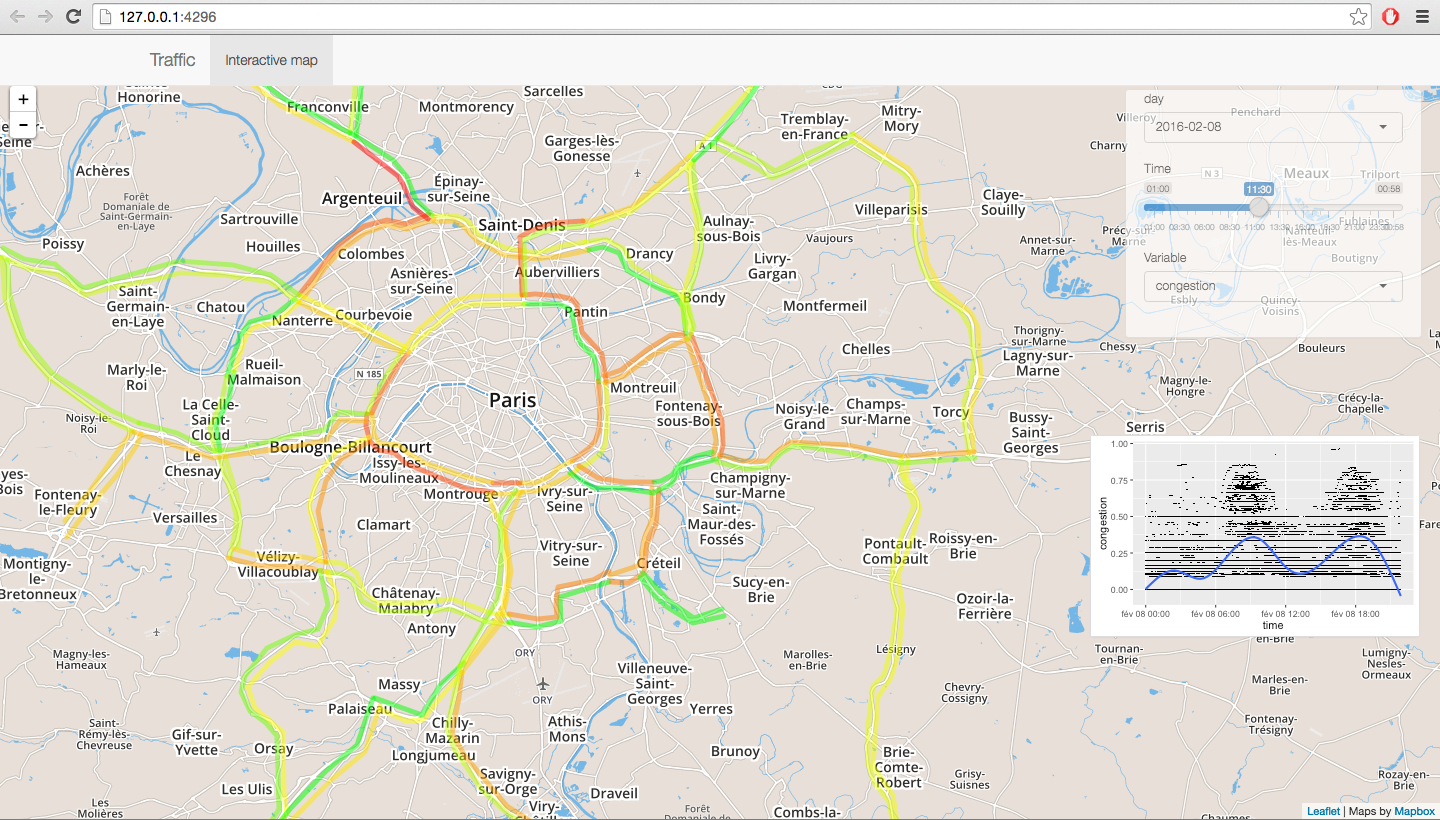
\includegraphics[width=\linewidth]{Figures/TransportationEquilibrium/gr1}
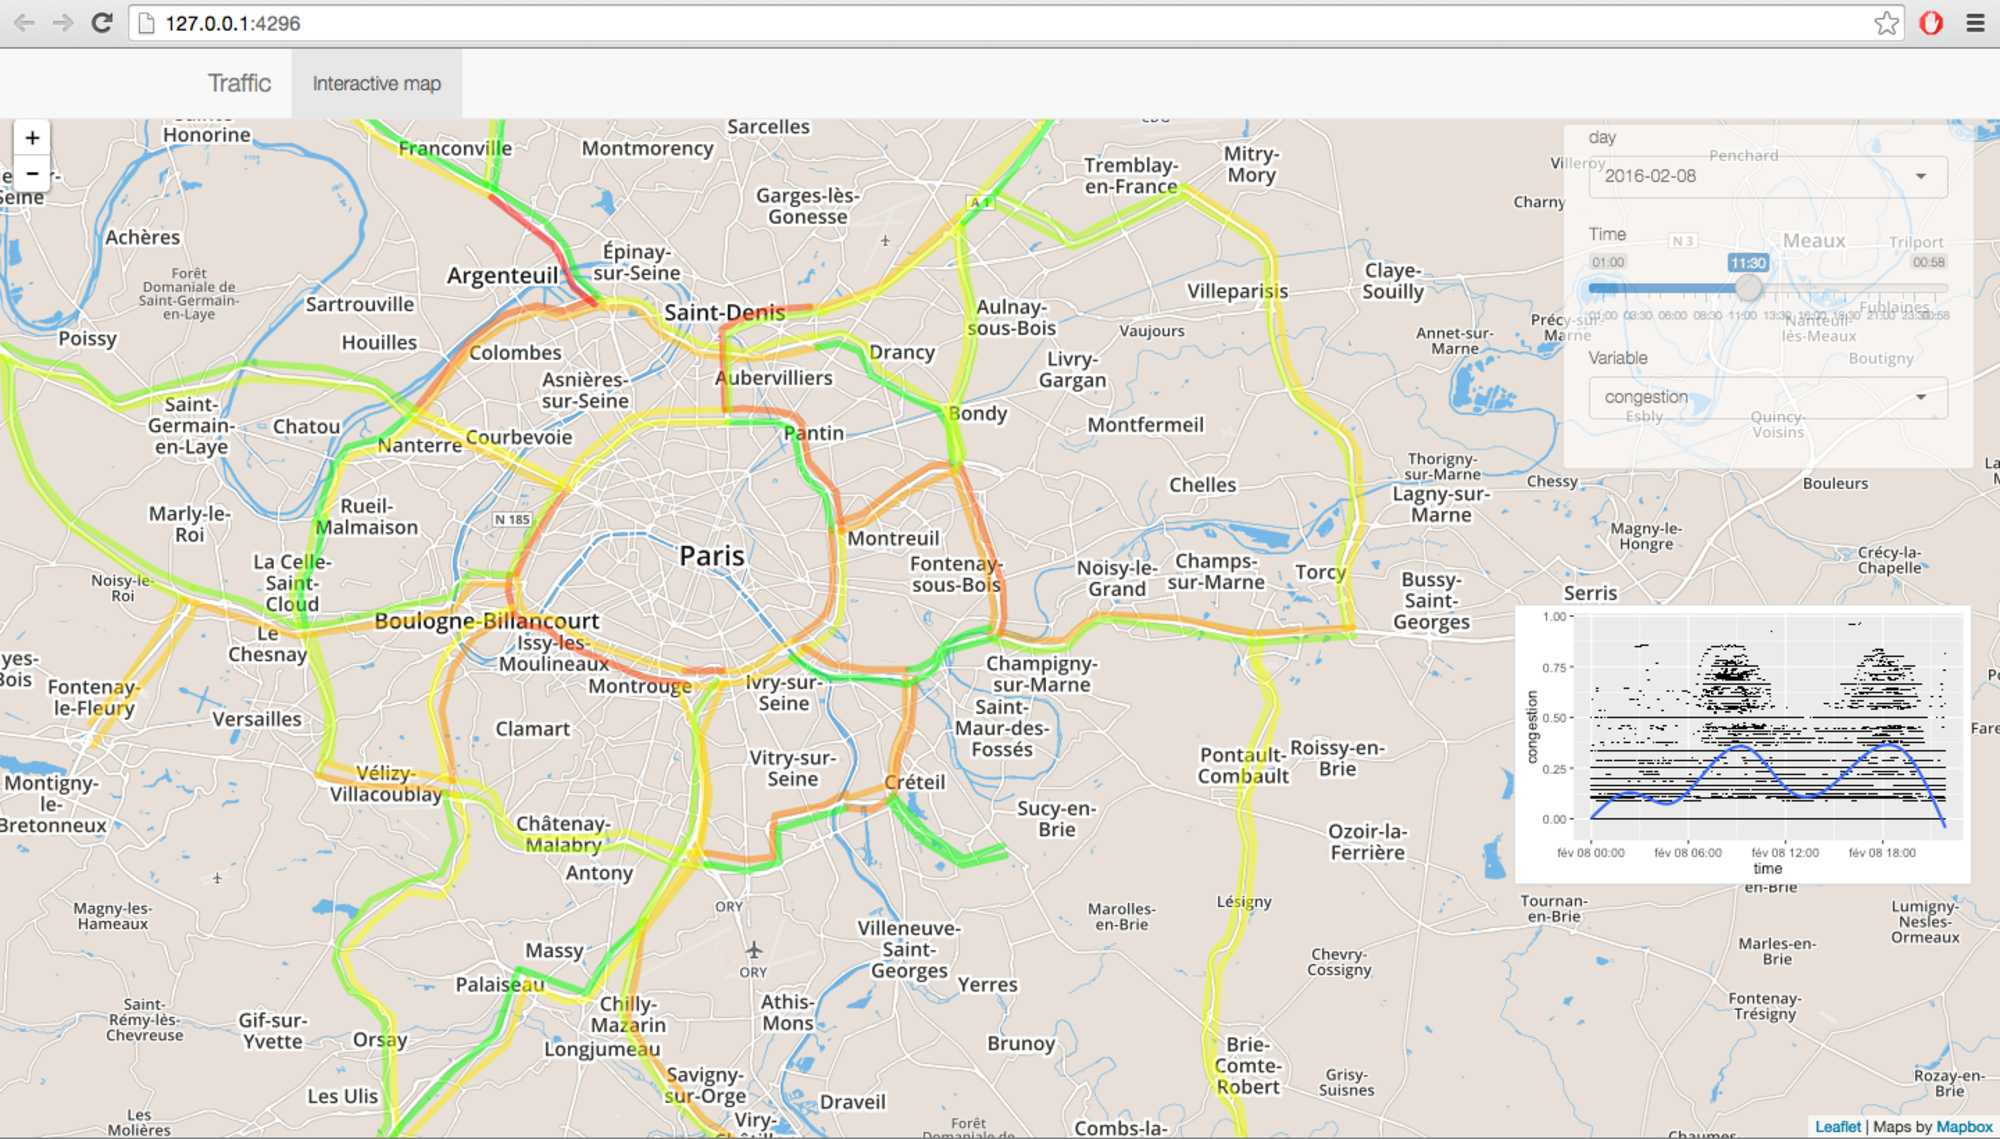
\includegraphics[width=\linewidth]{Figures/Final/8-1-2-fig-transportationequilibrium-fig-1.jpg}
\caption[Web-application for traffic data][Application web pour les données de trafic]{Capture of the web-application to explore spatio-temporal traffic data for Parisian region. It is possible to select date and time (precision of 15min on one month, reduced from initial dataset for performance purposes). A plot summarizes congestion patterns on the current day.\label{fig:transportationequilibrium:fig-1}}{\textbf{Capture de l'application web.} Nous avons développé celle-ci pour permettre l'exploration spatio-temporelle des données de trafic pour la région Parisienne. Il est possible de choisir date et heure (précision de 15min sur un mois, réduite par rapport au jeu de données initial pour des raisons de performance). Le graphe en insert résume les motifs de congestion pour la journée courante, en donnant en fonction du temps l'ensemble des valeurs (points noirs) et leur lissage (courbe bleue).\label{fig:transportationequilibrium:fig-1}}
\end{figure}
%%%%%%%%%%%%%%%%%%



%%%%%%%%%%%%%%%%%%%%%%%%
\paragraph{Spatio-temporal Variability of Travel Path}{Variabilité spatio-temporelle des trajets}


\bpar{
Following interactive exploration of data, we propose to quantify the spatial variability of congestion patterns to validate or invalidate the intuition that if equilibrium does exist in time, it is strongly dependent on space and localized. The variability in time and space of travel-time shortest paths is a first way to investigate flow stationarities from a game-theoretic point of view. Indeed, the static User Equilibrium is the stationary distribution of flows under which no user can improve its travel time by changing its route. A strong spatial variability of shortest paths at short time scales is thus evidence of non-stationarity, since a similar user will take a few time after a totally different route and not contribute to the same flow as a previous user. Such a variability is indeed observed on a non-negligible number of paths on each day of the dataset. We show in Figure~\ref{fig:fig-2} an example of extreme spatial variation of shortest path for a particular Origin-Destination pair.
}{
A la suite de l'exploration interactive des données, nous proposons de quantifier la variabilité spatiale des motifs de congestion pour valider ou invalider l'intuition que si l'équilibre existe par rapport au temps, il est fortement dépendant de l'espace et localisé. La variabilité spatio-temporelle des plus courts chemins de trajet est une première façon d'étudier la stationnarité des flux d'un point de vue de théorie des jeux. En effet, l'Equilibre Utilisateur Statique est la distribution stationnaire des flux sous laquelle aucun utilisateur ne peut augmenter son temps de trajet en changeant son itinéraire. Une forte variabilité spatiale des plus courts chemins sur de courtes échelles spatiales révèle ainsi une non-stationnarité, puisqu'un même utilisateur prendra un chemin complètement différent après un court laps de temps et ne contribuera plus au même flux que précédemment. Une telle variabilité est en effet observée sur un nombre non-négligeable de chemins pour chaque jour du jeu de données. La figure~\ref{fig:transportationequilibrium:fig-2} montre un exemple de variation spatiale extrême d'un trajet pour une paire Origine-Destination particulière.
}

\bpar{
The systematic exploration of travel time variability across the whole dataset, and associated travel distance, confirms, as described in Figure 3, that travel time absolute variability has often high values of its maximum across OD pairs, up to 25 minutes with a temporal local mean around 10min. Corresponding spatial variability produces detours up to 35km.
}{
L'exploration systématique de la variabilité du temps de trajet sur l'ensemble du jeu de données, et des distances de trajet associées, confirme, comme présenté en figure~\label{fig:transportationequilibrium:fig-3}, que la variation absolue du temps de trajet présente fréquemment une forte variation de son maximum sur l'ensemble des paires O-D, jusqu'à 25 minutes avec une moyenne temporelle locale autour de 10 minutes. La variabilité spatiale correspondante entraine des détours allant jusqu'à 35km.
}


%%%%%%%%%%%%%%%%%%%
\begin{figure}
%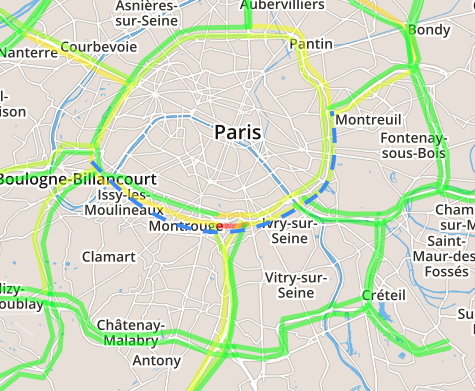
\includegraphics[width=0.47\linewidth]{Figures/TransportationEquilibrium/gr21}
%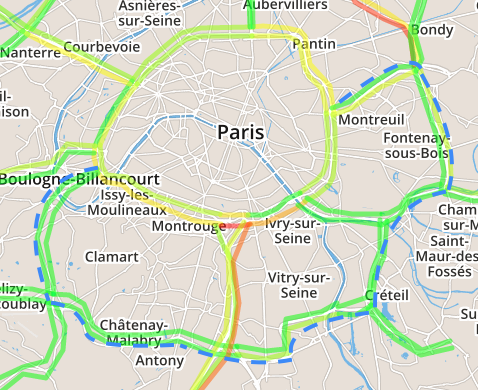
\includegraphics[width=0.47\linewidth]{Figures/TransportationEquilibrium/gr22}
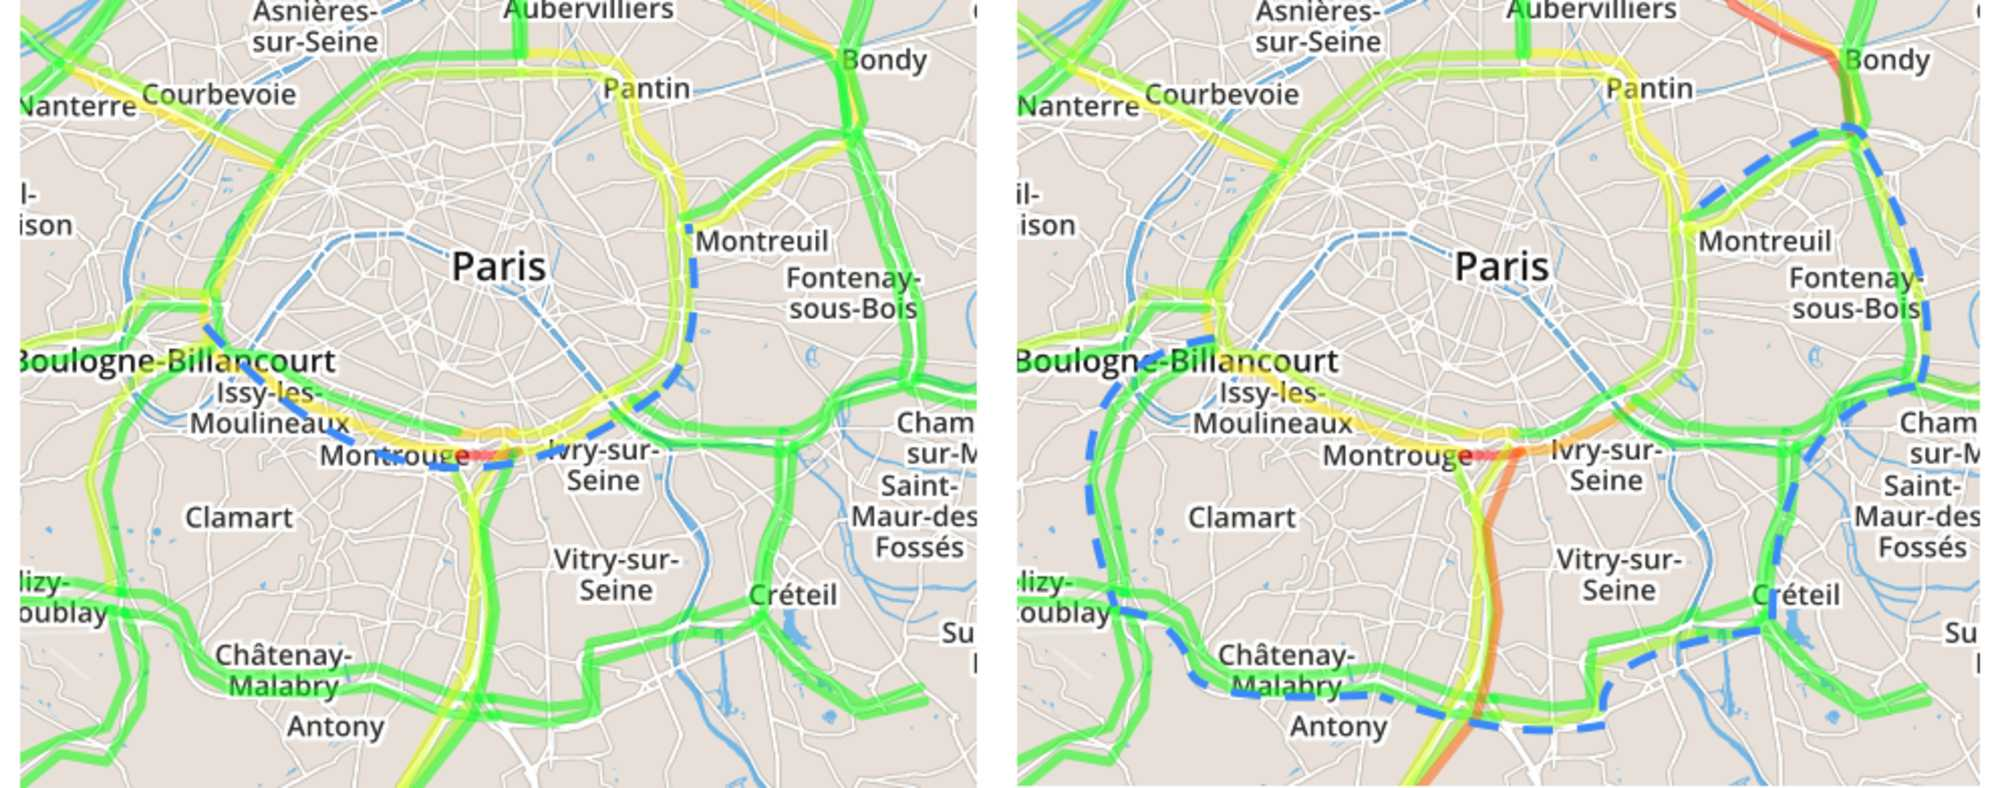
\includegraphics[width=\linewidth]{Figures/Final/8-1-2-fig-transportationequilibrium-fig-2.jpg}
\caption[Spatial variability of shortest paths][Variabilité spatiale des plus courts chemins]{Spatial variability of travel-time shortest path (shortest path trajectory in dotted blue). In an interval of only 10 minutes, between 11/02/2016 00:06 (left) and 11/02/2016 00:16 (right), the shortest path between \emph{Porte d'Auteuil} (West) and \emph{Porte de Bagnolet} (East), increases in effective distance of $\simeq 37$km (with an increase in travel time of only 6min), due to a strong disruption on the ring of Paris.\label{fig:fig-2}}{\textbf{Variabilité spatiale d'un plus court chemin en temps de trajet.} Le trajet du plus court chemin est donné en pointillé bleu. Dans un intervalle de seulement 10 minutes, entre le 11/02/2016 00:06 (à gauche) et le 11/02/2016 00:16 (à droite), le plus court chemin entre Porte d'Auteuil à l'ouest et Porte de Bagnolet à l'est, augmente en distance effective de $\simeq 37$km (avec une augmentation du temps de trajet de seulement 6 minutes), à cause d'une forte perturbation sur le périphérique parisien.\label{fig:transportationequilibrium:fig-2}}
\end{figure}
%%%%%%%%%%%%%%%%%%%



%%%%%%%%%%%%%%%%%%%
\begin{figure}
%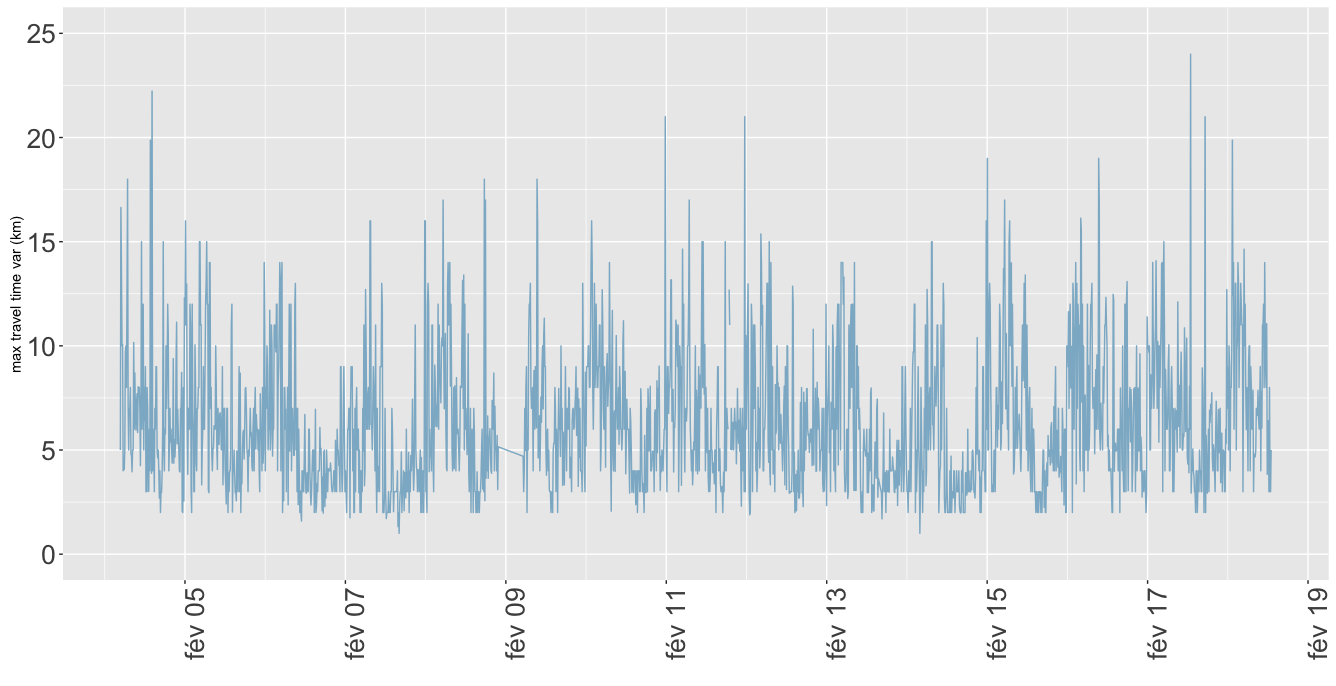
\includegraphics[width=\linewidth]{Figures/TransportationEquilibrium/gr31}
%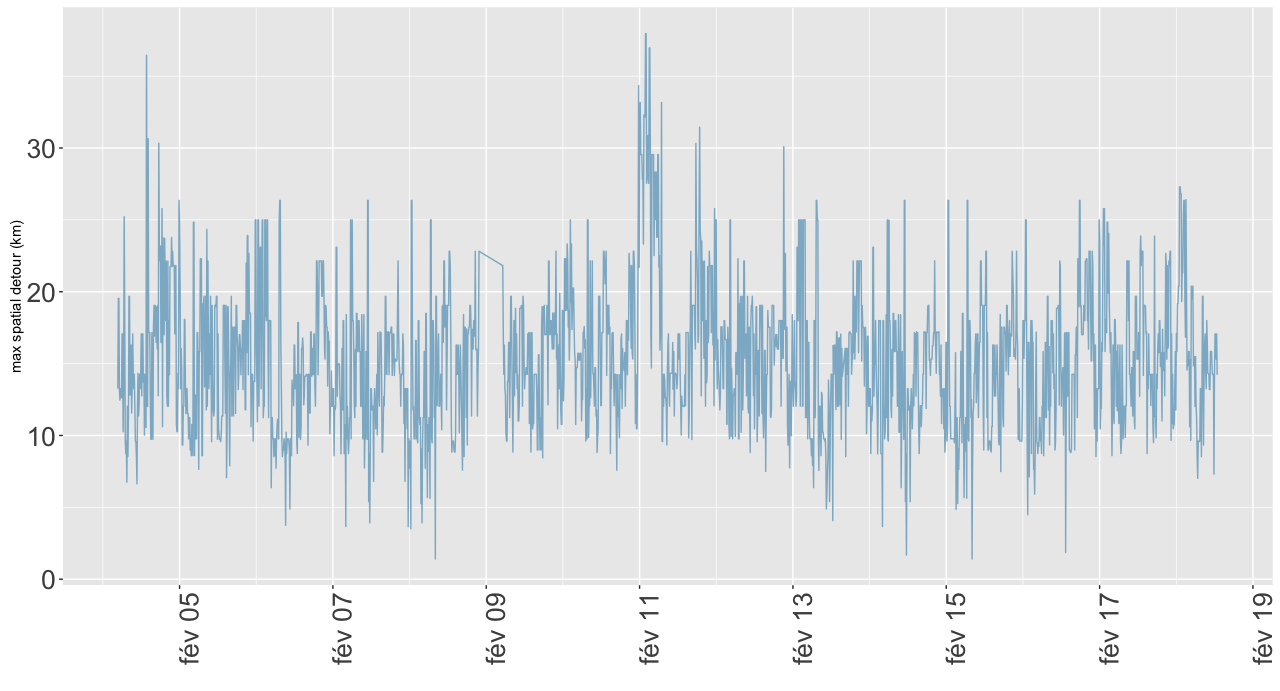
\includegraphics[width=\linewidth]{Figures/TransportationEquilibrium/gr32}
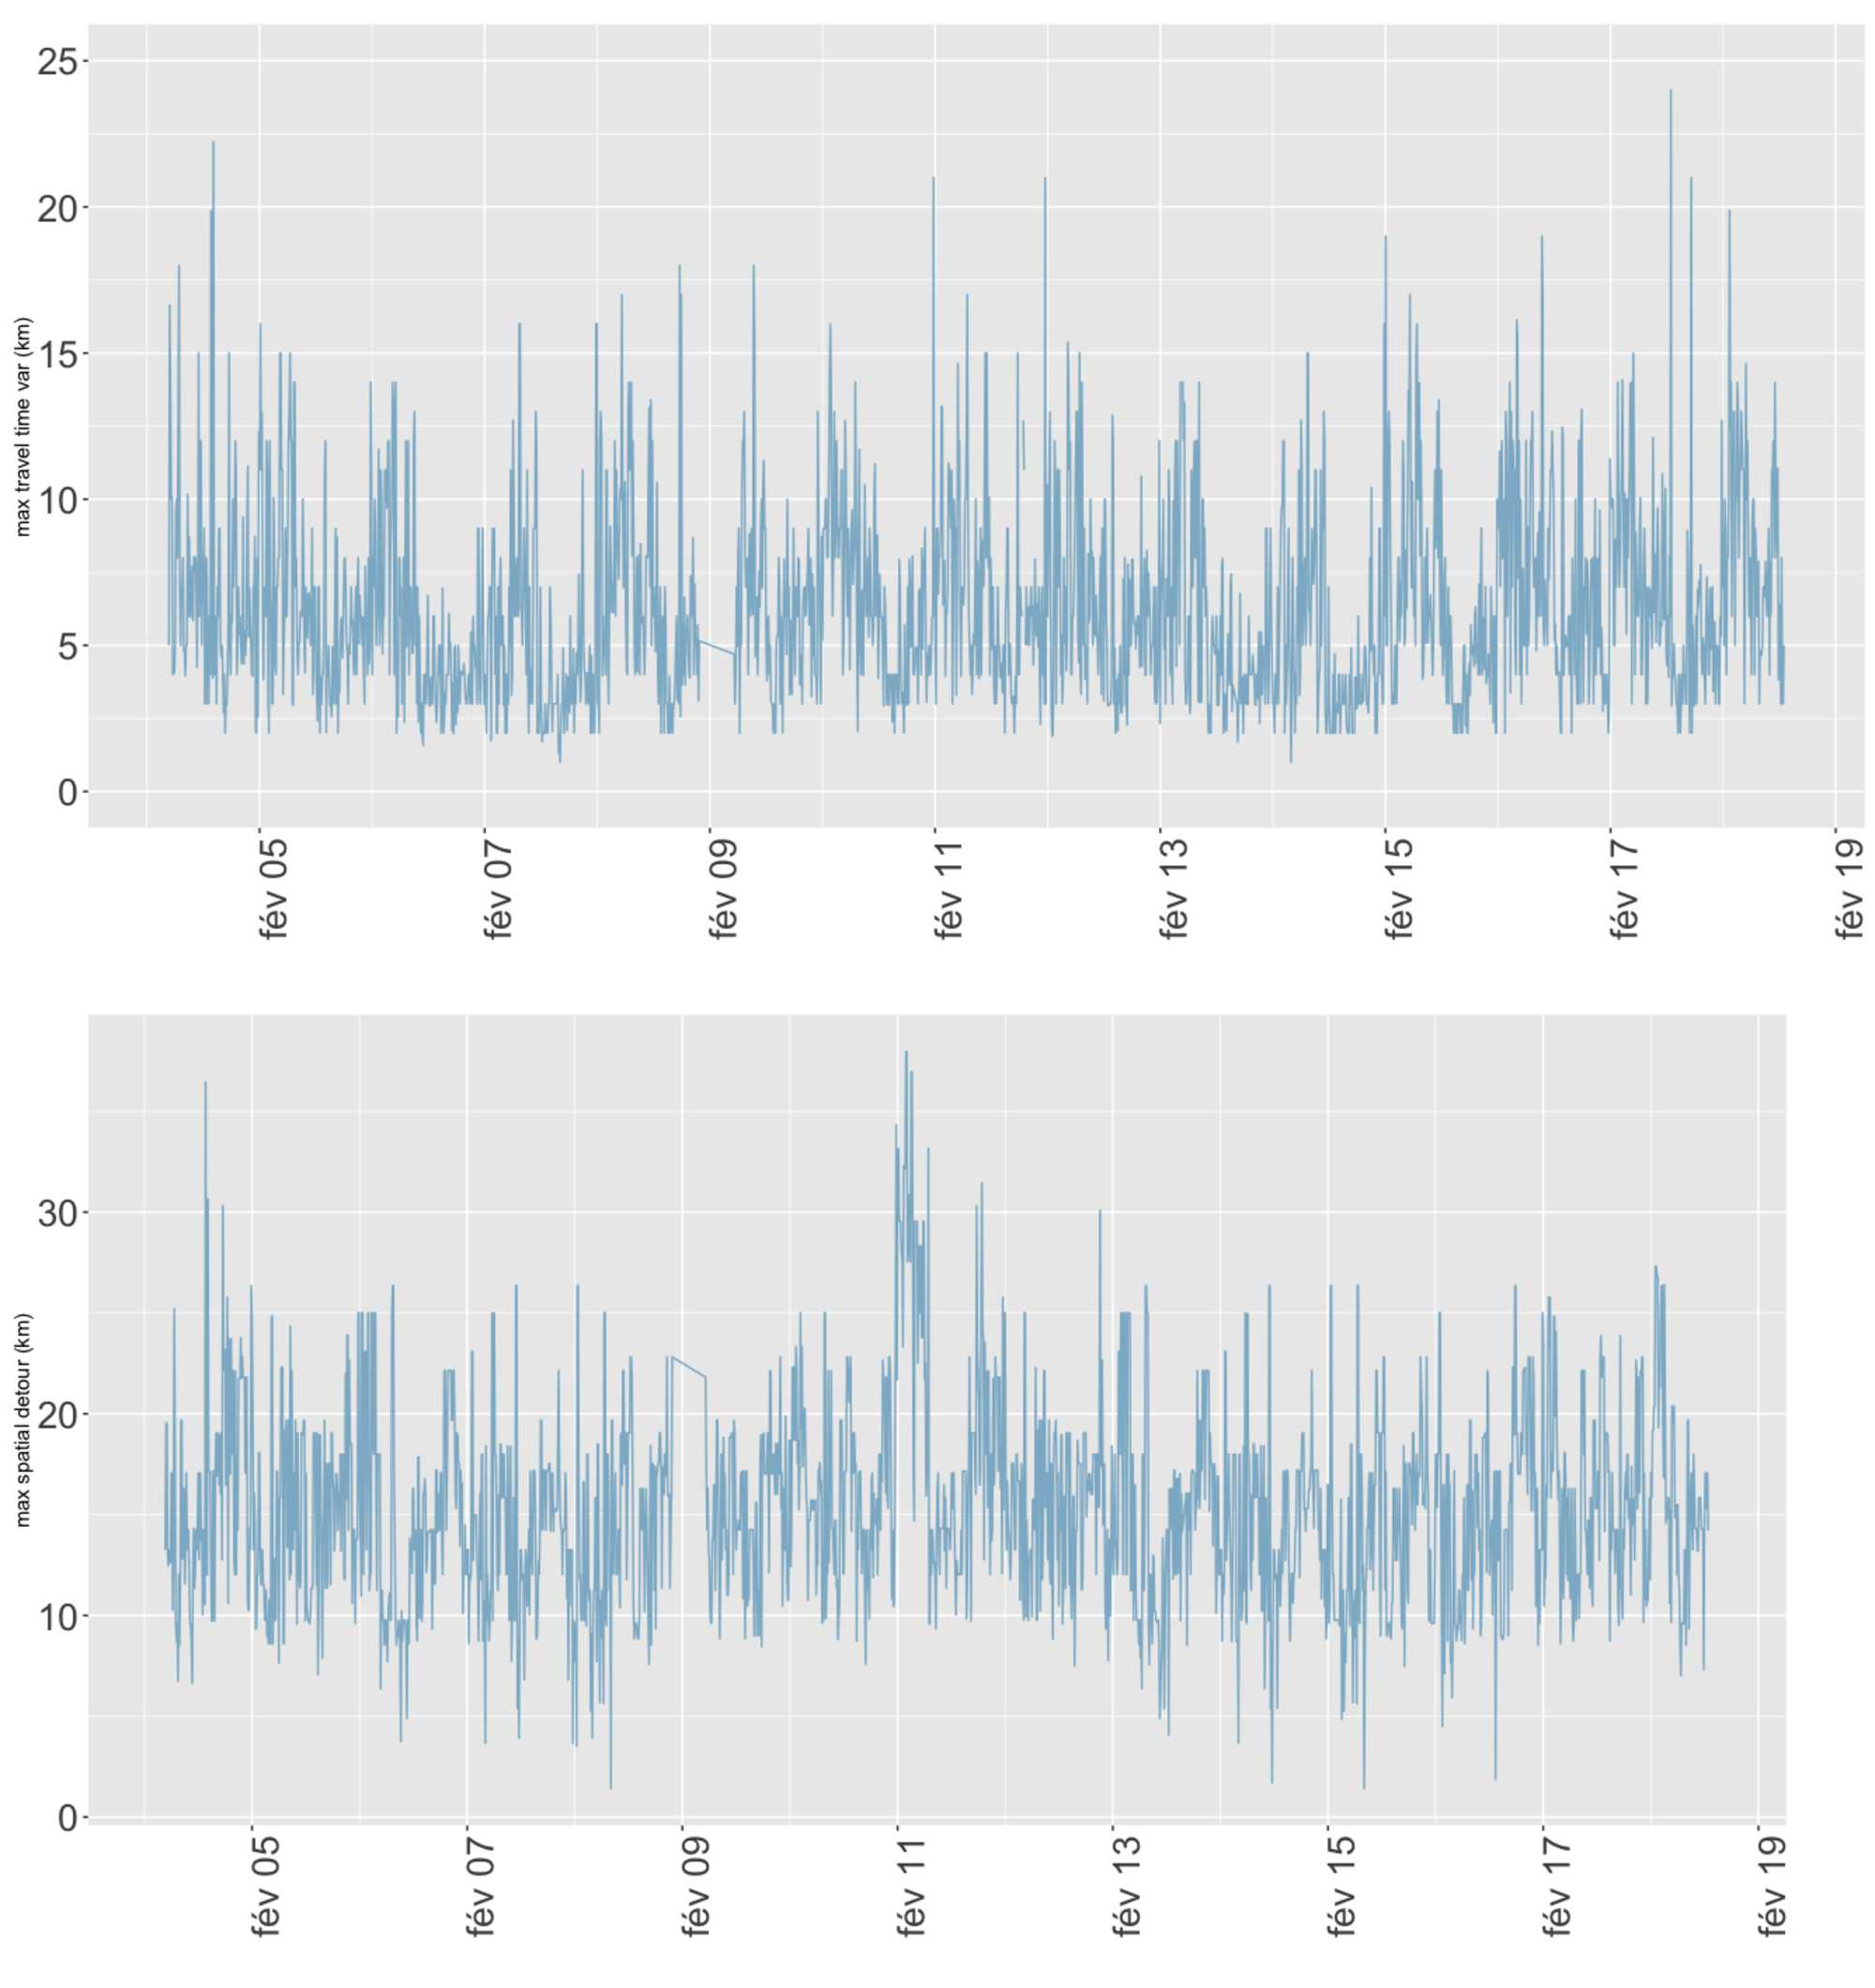
\includegraphics[width=\linewidth]{Figures/Final/8-1-2-fig-transportationequilibrium-fig-3.jpg}
\caption[Variability of travel time and distance][Variabilité des temps de trajet]{Travel time (top) in min and corresponding travel distance (bottom) maximal variability on a two weeks sample. We plot the maximal on all OD pairs of the absolute variability between two consecutive time steps. Peak hours imply a high time travel variability up to 25 minutes and a path length variability up to 35km.\label{fig:transportationequilibrium:fig-3}}{\textbf{Variabilité des temps de trajet.} Variabilité maximale du temps de trajet (\textit{Haut}) en minutes et de la distance de trajet correspondante (\textit{Bas}) pour un échantillon de deux semaines. Le graphe représente le maximum sur l'ensemble des paires Origine-Destination de la variabilité absolue entre deux pas de temps consécutifs. Les heures de pointe induisent une forte variabilité du temps de trajet, allant jusqu'à 25 minutes et une variabilité de distance jusqu'à 35km.\label{fig:transportationequilibrium:fig-3}}
\end{figure}
%%%%%%%%%%%%%%%%%%%




%%%%%%%%%%%%%%%%%%%
\paragraph{Stability of Network measures}{Stabilité des mesures de réseau}

\bpar{
The variability of potential trajectories observed in the previous section can be confirmed by studying the variability of network properties. In particular, network topological measures capture global patterns of a transportation network. Centrality and node connectivity measures are classical indicators in transportation network description as recalled in~\cite{bavoux2005geographie}. The transportation literature has developed elaborated and operational network measures, such as network robustness measures to identify critical links and measure overall network resilience to disruptions (an example among many is the Network Trip Robustness index introduced in~\cite{sullivan2010identifying}).
}{
La variabilité des trajectoires potentielles observée dans la section précédente peut être confirmée par l'étude de la variabilité des propriétés du réseau. En particulier, les mesures topologiques de réseau capturent les motifs globaux dans un réseau de transport. Les mesures de centralité et de connectivité des noeuds sont des indicateurs classiques pour la description des réseaux de transport comme rappelé par~\cite{bavoux2005geographie}. La littérature en transports a développé des mesures de réseau élaborées et opérationnelles, comme des mesures de robustesse pour identifier les liens critiques et mesurer la résilience globale du réseau aux perturbations (un exemple parmi d'autres est l'indice de \emph{Robustesse du Réseau Effective} introduit dans ~\cite{sullivan2010identifying}).
}



\bpar{
More precisely, we study the betweenness centrality of the transportation network, defined for a node as the number of shortest paths going through the node, i.e. by the equation

%%%%%%%%%%%%%%%
% equation betweeness
\begin{equation}
b_i = \frac{1}{N(N-1)}\cdot \sum_{o\neq d \in V}\mathbbm{1}_{i\in p(o\rightarrow d)}
\end{equation}
%%%%%%%%%%%%%%%

where $V$ is the set of network vertices of size $N$, and $p(o\rightarrow d)$ is the set of nodes on the shortest path between vertices o and d (the shortest path being computed with effective travel times). This index is more relevant to our purpose than other measures of centrality such as closeness centrality that does not include potential congestion as betweenness centrality does.
}{
Plus précisément, nous étudions la centralité de chemin du réseau de transport, défini pour un noeud comme le nombre de plus courts chemins passant par celui-ci, i.e. par l'équation

%%%%%%%%%%%%%%%
% equation betweeness
\begin{equation}
b_i = \frac{1}{N(N-1)}\cdot \sum_{o\neq d \in V}\mathbbm{1}_{i\in p(o\rightarrow d)}
\end{equation}
%%%%%%%%%%%%%%%

où $V$ est l'ensemble des sommets du réseau de taille $N$, et $p(o\rightarrow d)$ est l'ensemble des noeuds sur le plus court chemin entre les sommets $o$ et $d$ (le plus court chemin étant calculé avec le temps de trajet effectif). Cette mesure de centralité est plus adaptée que d'autres dans notre cas, comme la centralité de proximité qui n'inclut pas la congestion potentielle comme la centralité de chemin.
}



\bpar{
We show in Figure 4 the relative absolute variation of maximal betweenness centrality for the same time window than previous empirical indicators. More precisely we plot the value of

%%%%%%%%%%%%%%%
% eq relative variability
\begin{equation}
\Delta b(t) = \frac{\left|\max_i (b_i(t + \Delta t)) - \max_i (b_i(t))\right|}{\max_i (b_i(t))}
\end{equation}
%%%%%%%%%%%%%%%



where $\Delta t$ is the time step of the dataset (the smallest time window on which we can capture variability). This absolute relative variation has a direct meaning : a variation of 20\% (which is attained a significant number of times as shown in Fig.~\ref{fig:fig-4}) means that in case of a negative variation, at least this proportion of potential travels have changed route and the local potential congestion has decrease of the same proportion. In the case of a positive variation, a single node has captured at least 20\% of travels. Under the assumption (that we do not try to verify in this work and assume to be also not verified as shown by~\cite{zhu2010people}, but that we use as a tool to give an idea of the concrete meaning of betweenness variability) that users rationally take the shortest path and assuming that a majority of travels are realized such a variation in centrality imply a similar variation in effective flows, leading to the conclusion that they can not be stationary in time (at least at a scale larger than $\Delta t$) nor in space.
}{
Nous montrons en Fig.~\ref{fig:transportationequilibrium:fig-4} la variation relative absolue du maximum de la centralité de chemin, pour la même fenêtre temporelle que les indicateurs empiriques précédents. Plus précisément, elle est définie par :


%%%%%%%%%%%%%%%
% eq relative variability
\begin{equation}
\Delta b(t) = \frac{\left|\max_i (b_i(t + \Delta t)) - \max_i (b_i(t))\right|}{\max_i (b_i(t))}
\end{equation}
%%%%%%%%%%%%%%%


où $\Delta t$ est le pas de temps du jeu de données (la plus petite fenêtre temporelle sur laquelle une variabilité peut être capturée). Cette variation relative absolue a une signification directe : une variation de 20\% (qui est atteinte un nombre significatif de fois comme montré en Figure~\ref{fig:transportationequilibrium:fig-4}) implique dans le cas d'une variation négative, qu'au moins cette proportion de trajectoires potentielles ont changé et que la potentielle congestion locale a décru de la même proportion. Dans le cas d'une variation positive, un seul noeud a capturé au moins 20\% des trajets.

Sous l'hypothèse (qu'on ne tente pas de vérifier ici et qu'on peut également supposer non vérifiée comme montré par~\cite{zhu2010people}, mais que l'on utilise comme un outil pour donner une intuition sur la signification concrète de la variabilité de la centralité) que les utilisateurs choisissent rationnellement le plus court chemin, et supposant que la majorité des trajets est réalisée, une telle variation de la centralité implique une variation similaire dans les flux effectifs, conduisant à la conclusion qu'ils ne peuvent être stationnaires ni dans le temps (au moins sur une échelle plus grande que $\Delta t$) ni dans l'espace.
}




%%%%%%%%%%%%%%%%%%%
\begin{figure}
%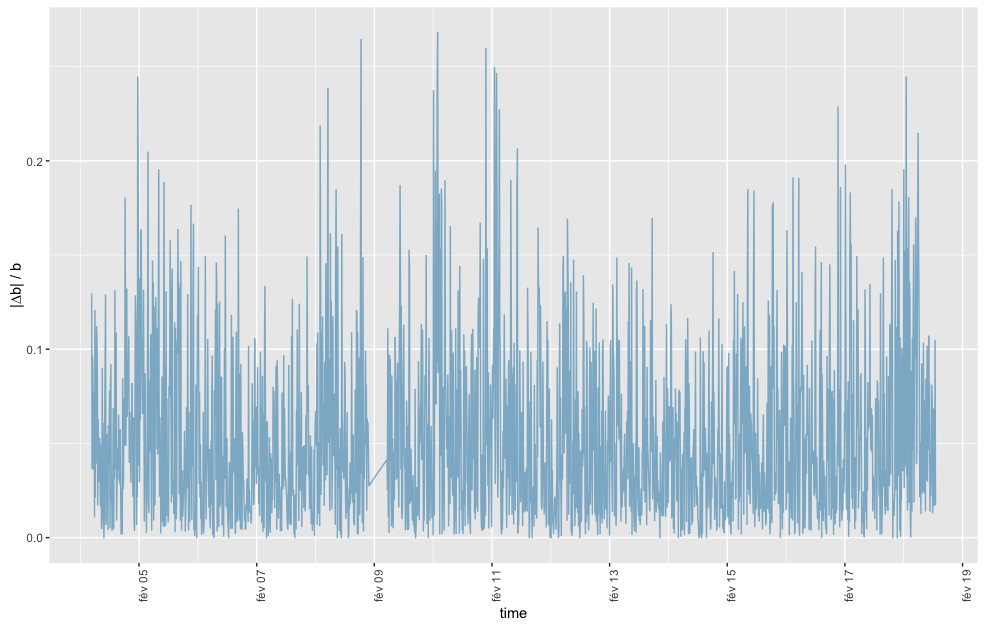
\includegraphics[width=\linewidth]{Figures/TransportationEquilibrium/gr4}
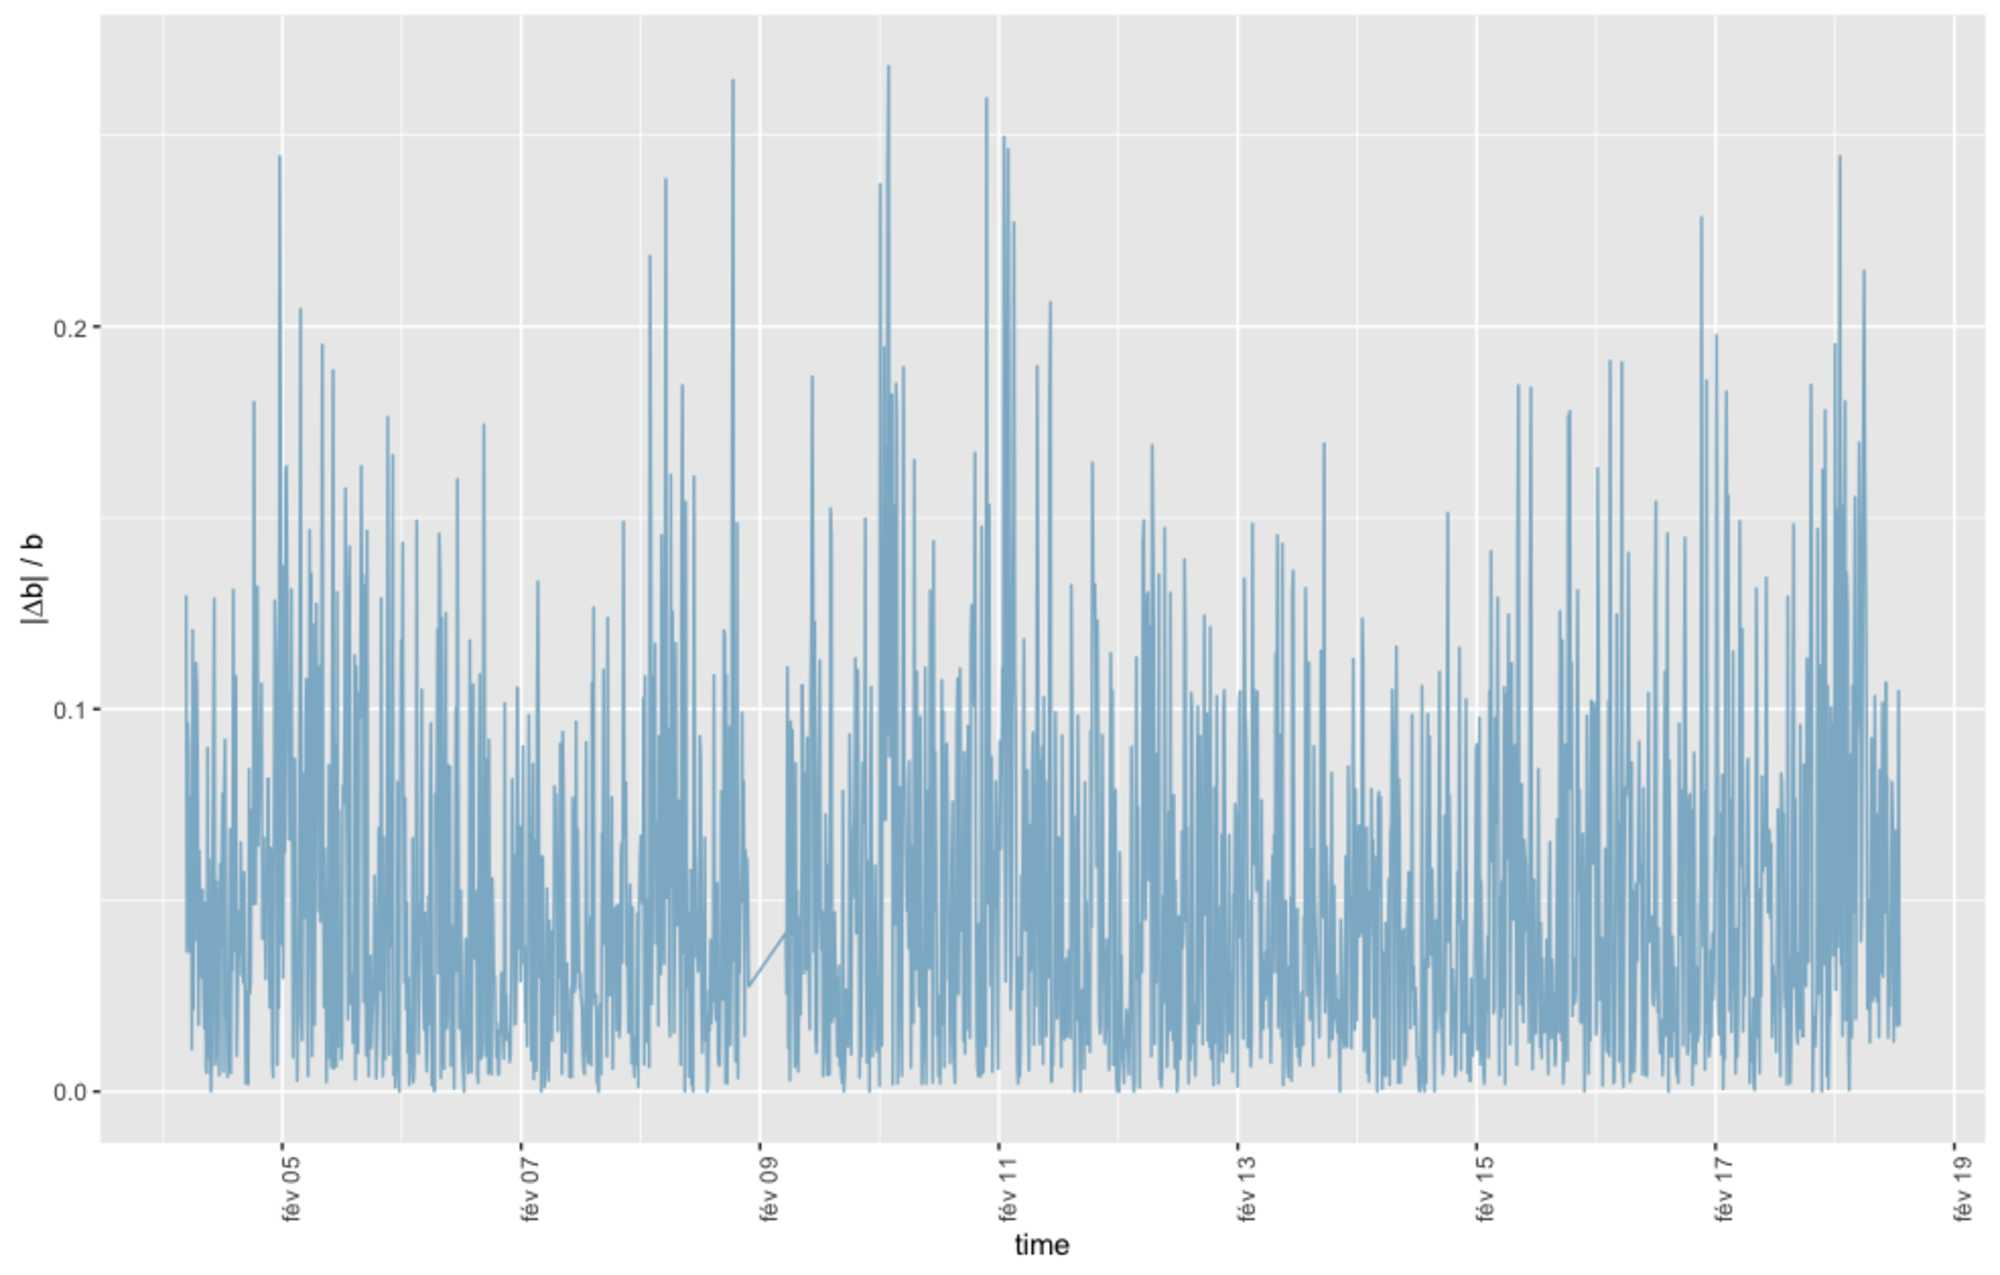
\includegraphics[width=\linewidth]{Figures/Final/8-1-2-fig-transportationequilibrium-fig-4.jpg}
\caption[Temporal stability of maximal betweenness centrality][Stabilité temporelle de la centralité]{Temporal stability of maximal betweenness centrality. We plot in time the normalized derivative of maximal betweenness centrality, that expresses its relative variations at each time step. The maximal value up to 25\% correspond to very strong network disruption on the concerned link, as it means that at least this proportion of travelers assumed to take this link in previous conditions should take a totally different path.\label{fig:transportationequilibrium:fig-4}}{\textbf{Stabilité temporelle du maximum de la centralité de chemin.} Le graphe montre dans le temps la dérivée normalisée du maximum de la centralité de chemin, qui capture ses variations relatives à chaque pas de temps. La valeur maximale de 25\% correspond à de très fortes perturbations du réseau sur les liens correspondants, puisque cela implique qu'au moins cette proportion d'utilisateurs prenant le lien dans des conditions précédentes doivent prendre un trajet complètement différent.\label{fig:transportationequilibrium:fig-4}}
\end{figure}
%%%%%%%%%%%%%%%%%%%




%%%%%%%%%%%%%%%%%%%
\paragraph{Spatial heterogeneity of equilibrium}{Hétérogénéité spatiale de l'équilibre}



\bpar{
To obtain a different insight into spatial variability of congestion patterns, we propose to use an index of spatial autocorrelation, the Moran index (defined e.g. in~\cite{tsai2005quantifying}). More generally used in spatial analysis with diverse applications from the study of urban form to the quantification of segregation, it can be applied to any spatial variable. It allows to establish neighborhood relations and unveils spatial local consistence of an equilibrium if applied on localized traffic variable. At a given point in space, local autocorrelation for variable c is computed by

%%%%%%%%%%%%
% Moran index def
\begin{equation}
\rho_i = \frac{1}{K}\cdot \sum_{i\neq j}{w_{ij}\cdot (c_i - \bar{c})(c_j - \bar{c})}
\end{equation}
%%%%%%%%%%%%

where $K$ is a normalization constant equal to the sum of spatial weights times variable variance and $\bar{c}$ is variable mean. In our case, we take spatial weights of the form $w_{ij} = \exp{\left(\frac{-d_{ij}}{d_0}\right)}$ with $d_0$ typical decay distance and compute the autocorrelation of link congestion localized at link center. We capture therefore spatial correlations within a radius of same order than decay distance around the point $i$. The mean on all points yields spatial autocorrelation index $I$. A stationarity in flows should yield some temporal stability of the index.
}{
Afin d'obtenir un point de vue différent sur la variabilité spatiale des motifs de congestion, nous proposons d'utiliser un indice d'auto-corrélation spatiale, l'indice de Moran (défini par exemple dans~\cite{tsai2005quantifying}). Utilisé plus généralement en analyse spatiale, avec diverses applications allant de l'étude de la forme urbaine à la quantification de la ségrégation, il peut être appliqué à toute variable spatiale. Il permet d'établir des relations de voisinage et révèle la consistence spatiale locale d'un équilibre s'il est appliqué à une variable de trafic localisée. À un point donné de l'espace, l'auto-corrélation locale pour la variable $c$ est calculée par

%%%%%%%%%%%%
% Moran index def
\begin{equation}
\rho_i = \frac{1}{K}\cdot \sum_{i\neq j}{w_{ij}\cdot (c_i - \bar{c})(c_j - \bar{c})}
\end{equation}
%%%%%%%%%%%%

où $K$ est une constante de normalisation égale à la somme des poids spatiaux fois la variance de la variable et $\bar{c}$ est la moyenne de la variable. Dans notre cas, nous choisissons des poids spatiaux de la forme $w_{ij} = \exp{\left(\frac{-d_{ij}}{d_0}\right)}$ avec $d_0$ distance typique de décroissance. L'auto-corrélation est calculée sur la congestion des liens, localisée au centre du lien. Elle capture ainsi les corrélations spatiales dans un rayon du même ordre que la distance de décroissance autour du point $i$. La moyenne sur l'ensemble des points fournit l'indice d'auto-corrélation spatiale $I$. Une stationnarité des flots devrait impliquer une stabilité temporelle de l'index. 
}



\bpar{
Figure~\ref{fig:transportationequilibrium:fig-5} presents temporal evolution of spatial autocorrelation for congestion. As expected, we have a strong decrease of autocorrelation with distance decay parameter, for both amplitude and temporal average. The high temporal variability implies short time scales for potential stationarity windows. When comparing with congestion (fitted to plot scale for readability) for 1km decay, we observe that high correlations coincide with off-peak hours, whereas peaks involve vanishing correlations. Our interpretation, combined with the observed variability of spatial patterns, is that peak hours correspond to chaotic behaviour of the system, as jams can emerge in any link: correlation thus vanishes as feasible phase space for a chaotic dynamical system is filled by trajectories in an uniform way what is equivalent to apparently independent random relative speeds.
}{
La figure~\ref{fig:transportationequilibrium:fig-5} présente l'évolution temporelle de l'auto-corrélation spatiale pour la congestion. Comme attendu, on observe une forte décroissance de l'auto-corrélation avec la distance de décroissance, à la fois sur l'amplitude et les moyennes temporelles. La forte variabilité temporelle implique de courtes échelles temporelles pour des fenêtres potentielles de stationnarité. Pour une distance de décroissance de 1km, en comparant l'auto-corrélation à la congestion (ajustée à l'échelle du graphe pour lisibilité), on observe que les fortes corrélations coincident avec les heures creuses, tandis que les heures de pointe correspondent à une décroissance des corrélations.

Notre interprétation, combinée avec la variabilité observée des motifs spatiaux, est que les heures de pointe correspondent à un comportement chaotique du système, puisque les bouchons peuvent émerger dans n'importe quel lien du réseau : la corrélation disparait alors puisque l'espace des phases atteignables pour un système dynamique chaotique est rempli uniformément par les trajectoires, de façon équivalente à des vitesses relatives qui apparaitraient comme aléatoires et indépendantes.
}



%%%%%%%%%%%%%%%%
\begin{figure}
%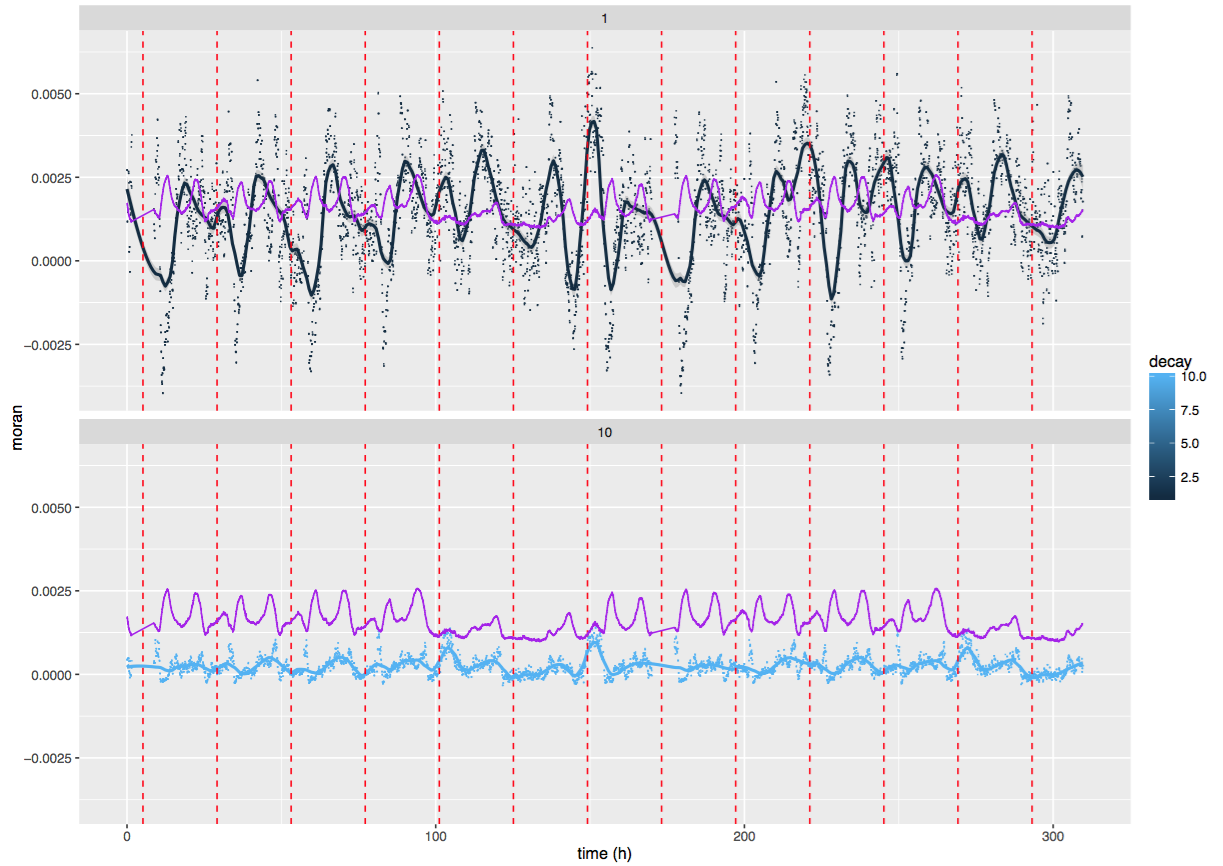
\includegraphics[width=\linewidth]{Figures/TransportationEquilibrium/gr5}
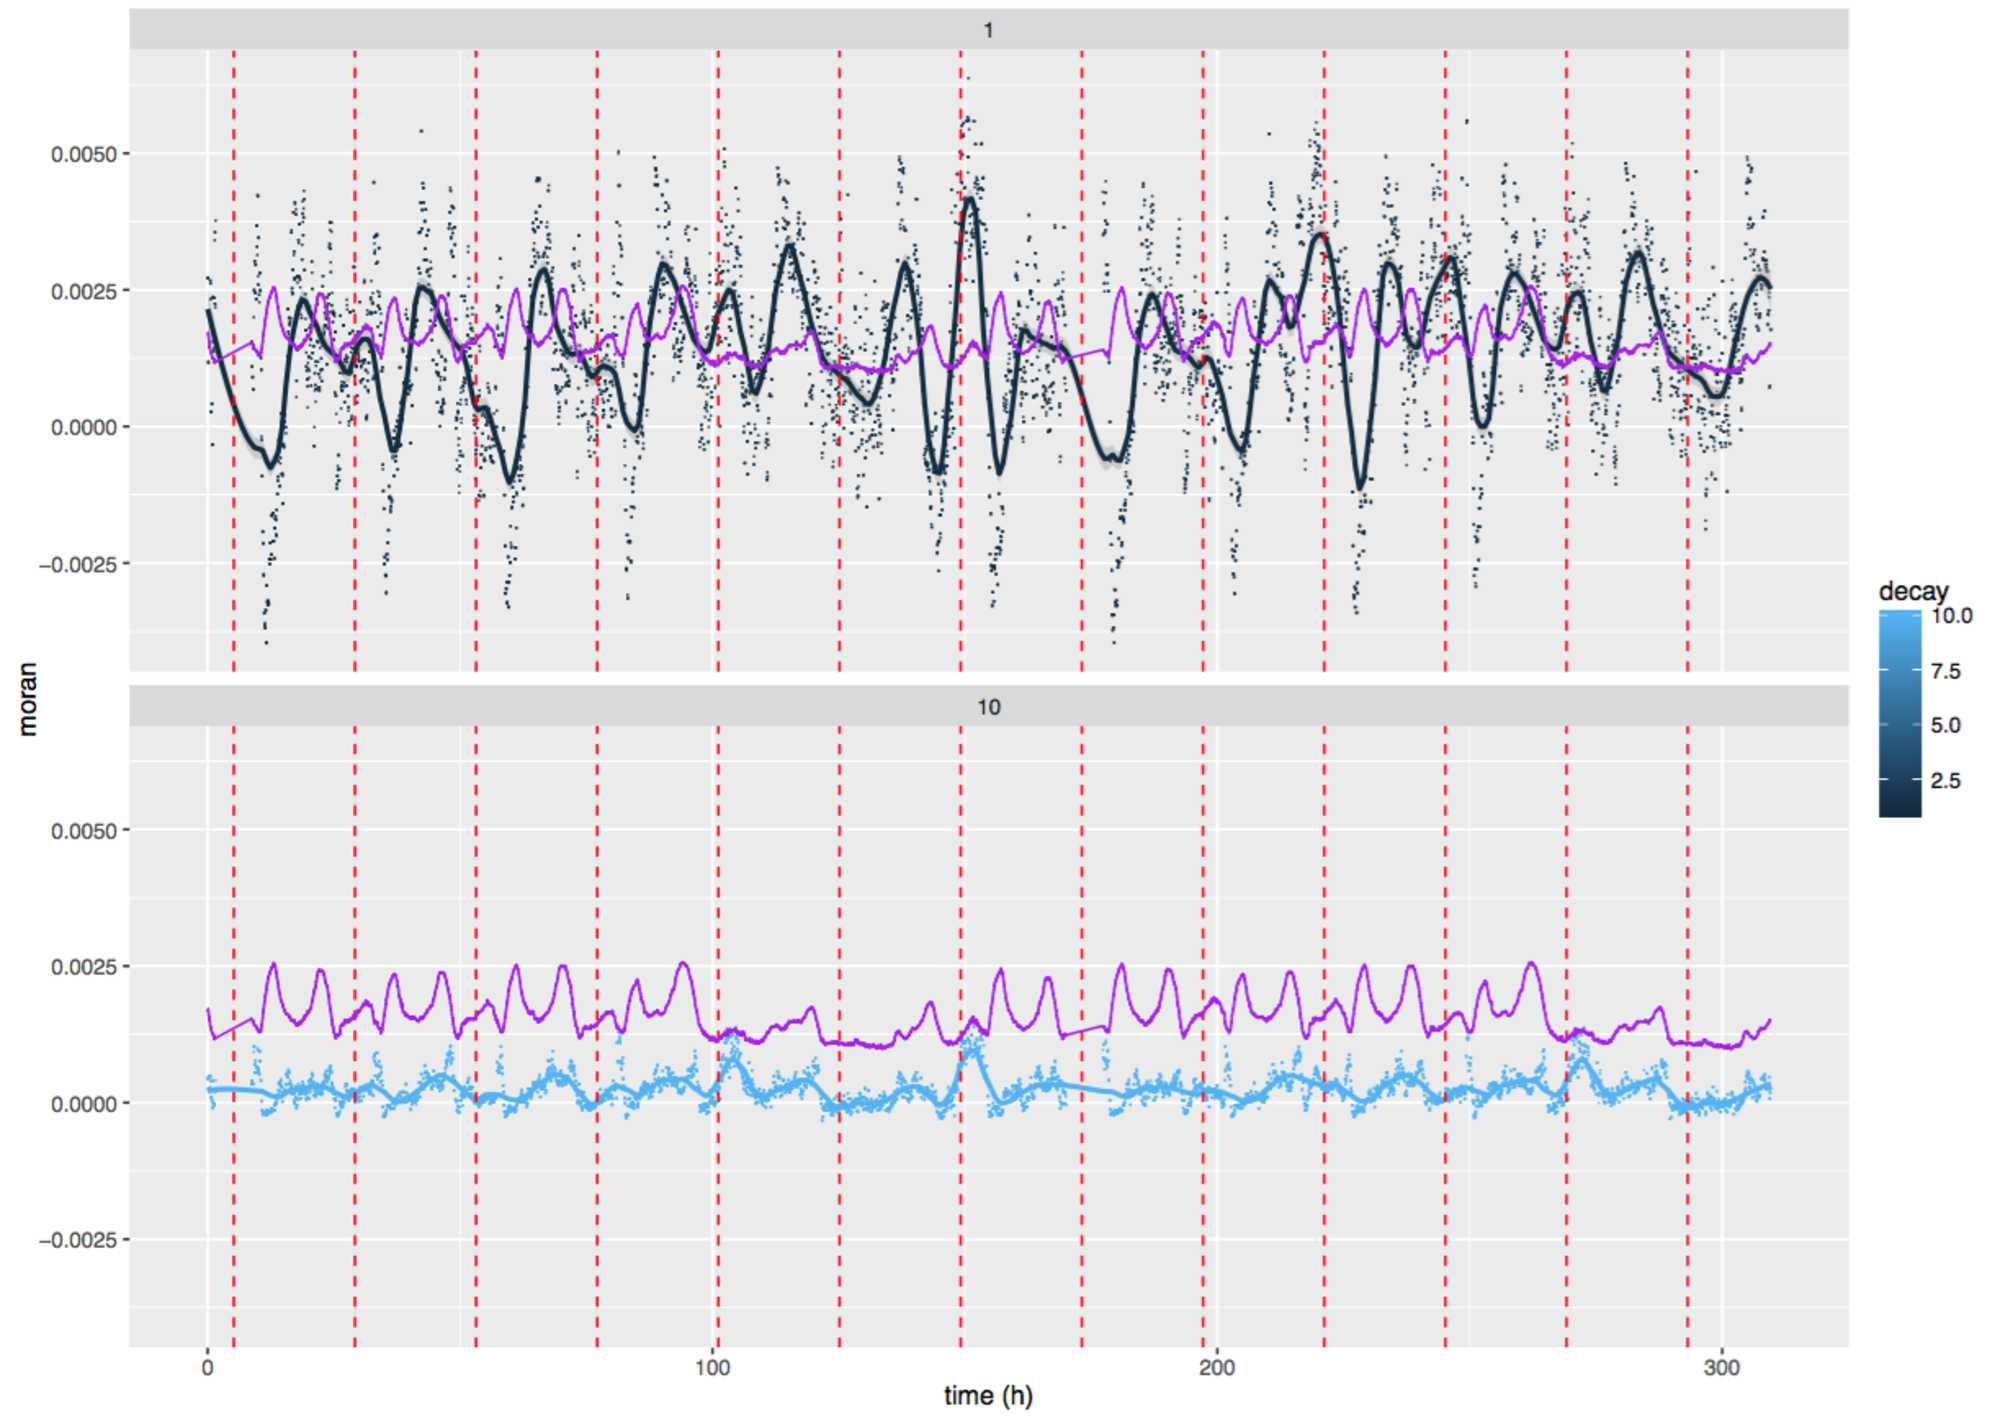
\includegraphics[width=\linewidth]{Figures/Final/8-1-2-fig-transportationequilibrium-fig-5.jpg}
\caption[Spatial auto-correlations for relative travel speed][Auto-corrélation spatiale de la congestion]{Spatial auto-correlations for relative travel speed on two weeks. We plot for varying value of decay parameter (1,10km) values of auto-correlation index in time. Intermediate values of decay parameter yield a rather continuous deformation between the two curves. Points are smoothed with a 2h span to ease reading. Vertical dotted lines correspond to midnight each day. Purple curve is relative speed fitted at scale to have a correspondence between auto-correlation variations and peak hours.\label{fig:transportationequilibrium:fig-5}}{\textbf{Auto-corrélations spatiales pour les vitesses relatives sur deux semaines.} Le graphe montre les valeurs de l'auto-corrélation dans le temps, pour des valeurs variables (1km ,10km) de la distance de décroissance (données en couleur et titre des graphes). les valeurs intermédiaires de la distance de décroissance donnent une déformation relativement continue entre ces deux extrêmes. Les points sont lissés sur une fenêtre temporelle de 2h pour faciliter la lecture. Les lignes pointillées verticales correspondent à minuit de chaque jour. La courbe violette donne la vitesse relative, ajustée à l'échelle pour établir la correspondance entre les heures de pointe et les variations de l'auto-corrélation.\label{fig:transportationequilibrium:fig-5}}
\end{figure}
%%%%%%%%%%%%%%%%







\bpar{
We have described an empirical study aimed at a simple but from our point of view necessary investigation of the existence of the static user equilibrium, more precisely of its stationarity in space and time on a metropolitan highway network. We constructed by data collection a traffic congestion dataset for the highway network of Greater Paris on 3 months with two minutes temporal granularity. The interactive exploration of the dataset with a web application allowing spatio-temporal data visualization helped to guide quantitative studies. Spatio-temporal variability of shortest paths and of network topology, in particular betweenness centrality, revealed that stationarity assumptions do not hold in general, what was confirmed by the study of spatial autocorrelation of network congestion. We suggest that our findings highlight a general need of higher connections between theoretical and empirical studies, as our work can discard misunderstandings on the theoretical static user equilibrium framework and guide the choice of potential applications.
}{
Nous avons décrit une étude empirique ayant pour but une approche simple, mais selon notre point de vue nécéssaire, de l'existence de l'équilibre utilisateur statique, plus précisément de sa stationnarité dans le temps et l'espace pour un réseau routier métropolitain principal. Un jeu de données de congestion du trafic est construite par collection de données, pour la métropole parisienne sur 3 mois avec une granularité temporelle de 2 minutes. L'exploration interactive du jeu de données via une application web permettant la visualisation spatio-temporelle aide à guider les analyses quantitatives. La variabilité spatio-temporelle des plus courts chemins et de la topologie du réseau, en particulier la centralité de chemin, révèle que l'hypothèse de stationnarité ne tient généralement pas, ce qui est confirmé par l'étude de l'auto-corrélation spatiale de la congestion du réseau.
%Nous suggérons que nos résultats soulignent un besoin général de plus grandes connexions entre les études théoriques et empiriques, puisque cette étude permet de chasser les incompréhensions théoriques sur l'Equilibre Utilisateur Statique, et guider le choix d'application potentielles.
}


\subsubsection{Perspective}{Mise en perspective}


\bpar{}{
Nous pouvons proposer une mise en perspective de ce travail au regard de notre problématique générale de la co-évolution. Les flux de trafic, qui sont représentatifs du fonctionnement du réseau de transport, sont générés par la distribution spatiale des activités et les comportements des agents microscopiques. Or nous venons de montrer que l'évolution temporelle de ces flux est complexe, rappelant des dynamiques chaotiques, ce qui peut être également compris comme un rôle essentiel de la non-linéarité dans l'émergence de la congestion.

Comme nous l'avons montré au chapitre~\ref{ch:thematic}, ces processus liés à la mobilité quotidienne sont probablement liés à un niveau propre de co-évolution entre réseaux et territoires (par exemple la congestion induisant une évolution du réseau, mais aussi éventuellement des relocalisations), que nous n'abordons pas en profondeur dans notre travail. Cette illustration montre ainsi (i) une illustration des interactions entre réseaux et territoires à cette échelle microscopique, suggérant l'existence d'effets complexes à cette échelle ; (ii) la difficulté éventuelle d'une modélisation de la co-évolution à cette échelle microscopique, vu les trajectoires chaotiques du système étudié.
}



\bpar{}{
Cette exploration empirique nous a permis d'illustrer d'une part la construction d'un jeu de données ouvertes pour combler l'absence de données, et d'autre part le rôle crucial de l'exploration interactive, qui doit rester combinée à des analyses plus poussées guidées par celle-ci.
}





\stars



Nous avons ainsi détaillé dans cette section certains enjeux liés à la reproductibilité et à la science ouverte, complétant notre positionnement spécifiques en termes de modélisation à un positionnement plus général correspondant à la pratique scientifique.


Nous allons finalement dans la dernière section qui suit encore monter en généralité et préciser nos positionnement épistémologiques, c'est à dire concernant les disciplines elles-mêmes et la production de connaissance. Cette étape sera cruciale, puisque notre positionnement au regard des systèmes sociaux et des systèmes biologiques permettra d'introduire les éléments fondamentaux pour une définition plus complète de la co-évolution.


\stars




















